\documentclass[12pt,a4paper]{article}

\usepackage[onehalfspacing]{setspace}
\usepackage{natbib}
 
\usepackage{float}
%f�r feststellen der figures und tables [H] dranschreiben
\usepackage{units}
%wird so benutzt: 
%\unit[value/Zahl]{dimension/Einheit} oder 
%\unitfrac[value/Zahl]{dimension/Einheit num/Z�hler}{dimension/Einheit denum/Nenner} oder
%\nicefrac[fontcommand/Schriftart]{dimension/Einheit num/Z�hler}{dimension/Einheit denum/Nenner}
\usepackage{amssymb}
\usepackage{caption}
\usepackage{subcaption}

\usepackage{hyperref}

\usepackage[left=2cm,right=2cm,top=2cm,bottom=2cm]{geometry}
\usepackage[latin9]{inputenc}
\usepackage[ngerman]{babel}
\usepackage[T1]{fontenc}
\usepackage{lmodern}
\usepackage{amsmath}
\usepackage{graphicx}
\usepackage{textcomp}



\begin{document}

%deckblatt erstellen.

\begin{titlepage}

\begin{center}
% Oberer Teil der Titelseite:

\includegraphics[width=0.75\textwidth]{logo.png}\\[1cm]    	%Logo 

\textsc{\LARGE Bergische Universit\"at Wuppertal}\\[1.5cm]	%Institution

\textsc{\Large Fortgeschrittenen Praktikum}\\[0.5cm]				%Projekt


\newcommand{\HRule}{\rule{\linewidth}{0.5mm}}
\HRule \\[0.4cm]
{ \huge \bfseries Rutherford\\ Streuung von $\alpha$-Teilchen}\\[0.4cm]				%Titel

\HRule \\[1.5cm]

% Author und Tutor
\begin{minipage}{0.4\textwidth}
\begin{flushleft} \large
\emph{Verfasser:}\\
Henrik \textsc{J�rgens} \\
Frederik \textsc{Strothmann} \\
\end{flushleft}
\end{minipage}
\hfill
\begin{minipage}{0.4\textwidth}
\begin{flushright} \large
\emph{Tutoren:} \\
Max \textsc{Mustermann} \\
Max \textsc{Mustermann} \\
\end{flushright}
\end{minipage}

\vspace{1cm}

\begin{table}[H]
\centering
\begin{tabular}{|l|}
\hline \textbf{Abstract: } \\
Ziel des Versuches ist es, die Wechselwirkung von $\alpha$-Teilchen mit Materie zu untersuchen.\\
Die Aspekte Streuwinkel, Reichweite, Kernladung und Absorbtionsverhalten werden thematisiert.\\
\hline 
\end{tabular}
\end{table} 

\vspace{1cm}

\begin{table}[H]
\centering
\begin{tabular}{|c|c|c|}
\hline Dies & ist & ein \\ 
\hline Platz- & halter & f�r \\ 
\hline die & bewertungs & Tabelle \\ 
\hline 
\end{tabular} 
\end{table}

\vfill

% Unterer Teil der Seite/Datum
{\large \today}

\end{center}

\end{titlepage}

\newpage
\tableofcontents
\newpage

\bibliographystyle{plain}


\section{Einleitung}
%einleitung zu dem experiment.
%auf die einstellungen, die vor dem versuch gemacht werden, eingehen, oder auf eine anleitung dazu verweisen.
%---------------------------------------------------------------------------------------------
%hinter der einleitung kann der allgemeine theoretische hintergrund in einer zus�tzlichen section erkl�rt werden
In diesem Versuch werden Oberfl�chen verschiedener Proben mittels Rasttunnelmikroskopie auf deren Gitterstruktur und morphologische Eigenschaften untersucht. Elektronendichte, Oberfl�chenrauheit und die atomare Gitterstruktur k�nnen mit dem Rastertunnelmikroskop (RTM) analysiert werden. Der quantenmechanische Tunneleffekt wird genutzt, um leitende Materialien zu untersuchen. Indem zwischen einer einatomigen Platin-Iridum-Elektrode und der zu untersuchenden Probe eine Potentialdifferenz angelegt wird, kommt es abh�ngig von der Entfernung der Pt-Ir-Elektrode zur Probe und dessen Elektronendichte zu einem Tunnelstrom, welcher R�ckschl�sse auf die Struktur der Probe erlaubt. Die Elektronendichte der Oberfl�che kann durch systematisches Abrastern der Probe erfasst werden, sodass mithilfe verschiedener Modi (CC und CH: Constant Current und Constant Height) ein Bild der Materialoberfl�che entsteht.
\section{Theorie}
% Es sollen die wichtigsten theoretischen Formeln und Zusammenh�nge einmal ausf�hrlich erkl�rt werden
Es werden die theoretischen Grundlagen zur Bestimmung der Lebensdauer von Myonen besprochen.

\subsection{Standardmodell}
Das Standartmodell der Teilchenphysik drei der vier Grundlegenden Wechselwirkungen (WW), die schwache WW, die elektromagnetische WW und die Starke WW.
Die Kr�fte wechselwirken �ber Vektorbosonen, welche eine ganzzahligen Spin haben.
In Tabelle \ref{tab:ww} ist eine �bersicht der drei Kr�fte zu sehen.

\begin{table}[H]
\caption{In der Tabelle sind die Grundlegenden WW (au�er der Gravitation) und ihre Eigenschaften aufgetragen (entnommen \cite{povh} Seite 274)}
\label{tab:ww}
\centering
\begin{tabular}{|c|c|c|c|c|}
\hline Wechselwirkung & koppelt an & Austauschteilchen & $\frac{m_0}{GeV}$ & J$^P$ \\ 
\hline stark & Farbe & 8 Gluonen (g) & 0 & 1$^-$ \\ 
\hline elektromagnetisch & elektrische Ladung & Photon ($\gamma$) & 0 & 1$^-$ \\ 
\hline schwach & schwache Ladung & W$^\pm$, Z$^0$ & $\approx 10^2$ & 1 \\ 
\hline 
\end{tabular} 
\end{table}
Neben den Bosonen gibt es noch zwei weitere Fundamentale Teilchenarten die Quark und die Leptonen welche die Grundbausteine der Materie darstellen.
Beide geh�ren zu den Fermionen, haben also einen halbzahligen Spin. Leptonen und Quarks werden mit aufsteigender Masse in drei Generationen aufgeteilt.
In Tabelle \ref{tab:fermi} sind Quarks und Leptonen mit ihren Eigenschaften dargestellt.

\begin{table}[H]
\caption{�bersicht der Grundlegenden Eigenschaften von Quarks und Leptonen}
\label{tab:fermi}
\centering
\begin{tabular}{|p{2cm}|p{2cm}|p{2cm}|p{1cm}|p{3.5cm}|p{1cm}|}
	\hline
	Fermionen & \hspace{0.25cm} Familie \newline 1 \hspace{0.3cm} 2 \hspace{0.3cm} 3                                               & elektrische Ladung    & Farbe  & schwacher Isospin \newline rechtsh. \hspace{0.5cm} linksh. & Spin \\ \hline
	Leptonen  & $\nu_e$ \hspace{0.17cm} $\nu_\mu$ \hspace{0.17cm} $\nu_\tau$ \newline e \hspace{0.3cm} $\mu$ \hspace{0.3cm} $\tau$ & \hspace{0.6cm} 0 \newline  \hspace*{0.6cm} -1      & ------ & 1/2 \hspace{1.5cm} --- \newline \hspace*{2.4cm} 0          & 1/2  \\ \hline
	Quarks    & u \hspace{0.3cm} c \hspace{0.3cm} t \newline d \hspace{0.3cm} s \hspace{0.3cm} b                                   & \hspace*{0.2cm} +2/3 \newline \hspace*{0.3cm} -1/3 & r,g,b  & 1/2 \hspace{1.64cm} 0 \newline \hspace*{2.4cm} 0           & 1/2  \\ \hline
\end{tabular} 
\end{table}


\section{Versuchsaufbau}
%skizze zum versuchsaufbau (oder foto) einf�gen,   es muss erkl�rt werden wie das ganze funktioniert und welche speziellen einstellungen verwendet wurden (z.b. welche kn�pfe an den ger�ten f�r die messung verdreht wurden)
F�r den Versuch werden zwei verscheiden Vakuumkammern verwendet. Die erste Kammer  ist eine Rutherford-Streukammer, eine schematische Skizze ist in Abb. \ref{fig:kammer} zu sehen. Die Streukammer besteht aus einer Vakuumkammer, mit durchsichtigem Deckel. Ein Barometer, ein Bel�ftungsventil und ein Ventil mit Anschluss an die Vakuumpumpe sind an den Absperrhahn (3) angeschlossen. Der Halbleiterdetektor mit Kollimator (12,12.1) ist von innen an einer BNC-Buchse (2.1) montiert. Von au�en ist ein Vorverst�rker angeschlossen, die Daten werden von einem Digitalz�hler, der an einen Computer angeschlossen ist ausgelesen (siehe Abb. \ref{fig:aufbau}). Der Deckel der Streukammer hat einen Schwenkarm (7), an dem das $^{241}$Am-Pr�parat (7.1) , verschiedene Rahmen mit SpaltkKollimatoren (9) und Metallfolien (10) angebracht werden k�nnen. �ber einen Knopf (4) ist der Schwenkarm drehbar, der Winkel ist dabei �ber eine Skala (8) ablesbar. Zur Verf�gung stehen Spalte mit 1m und 5mm Breite sowie eine Goldfolie mit 2$\mu$m und eine Aluiminiumfolie mit 7$\mu$m Dicke.

\begin{figure}[H]
	\centering
  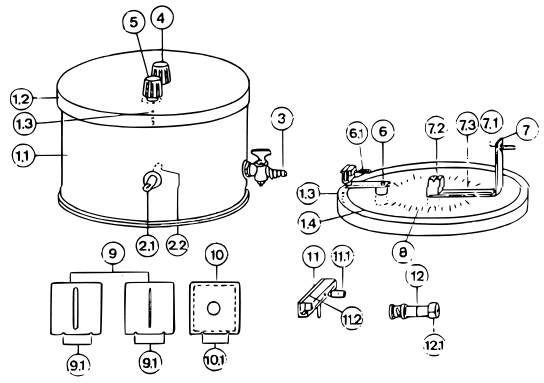
\includegraphics[scale=0.4]{streukammer.png}
	\caption{Schematischer Aufbau des Streukammer}
	\label{fig:kammer}
\end{figure}


\begin{figure}[H]
	\centering
  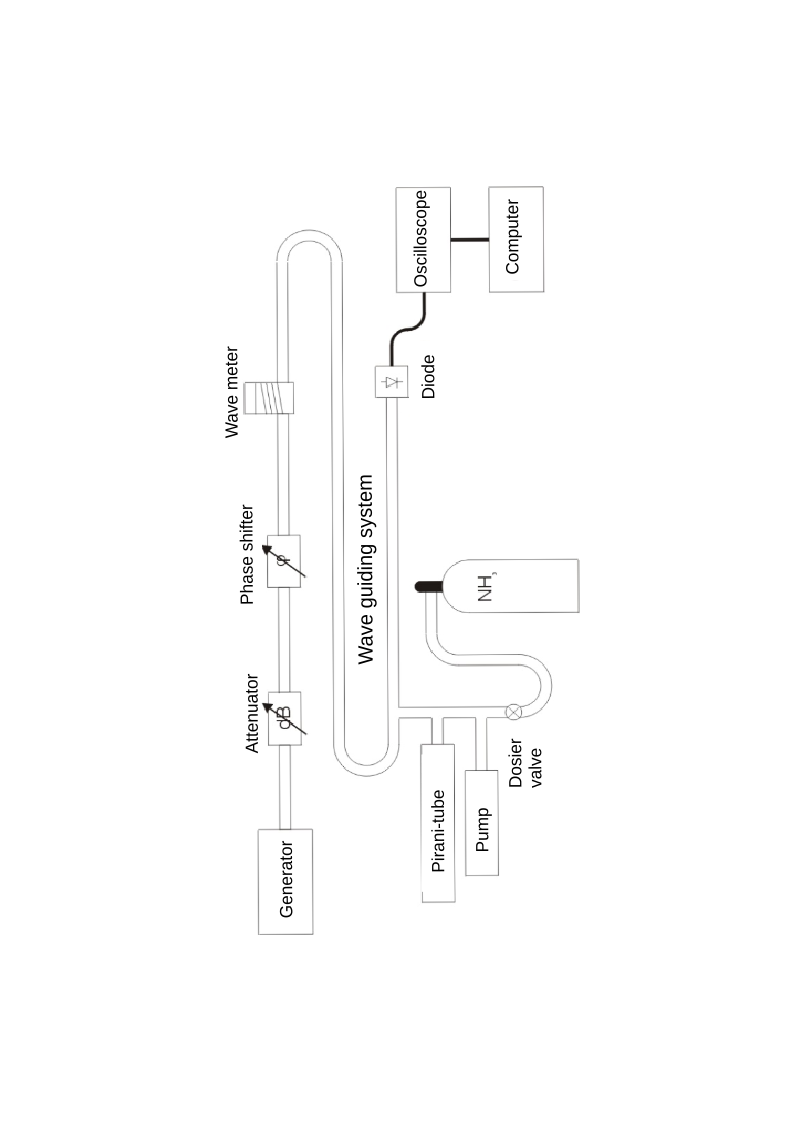
\includegraphics[scale=0.4]{aufbau.png}
	\caption{Schematischer Aufbau des Versuchsaufbaus}
	\label{fig:aufbau}
\end{figure}

Die zweite Kammer ist eine Vakuumkammer, mit einer optischen Bank, zu befestigen der radioaktiven Quelle. Sie wird f�r die Bestimmung der Reichweite von $\alpha$-Strahlung und die Untersuchung von Absorbtion durch verschiedenen Medien verwendet. Der Detektor ist an einen PC angeschlossen mit dem die Messdaten aufgenommen werden.
\section{Versuchsdurchf�hrung}
%erkl�ren, !was! wir machen, !warum! wir das machen und mit welchem ziel
%(wichtig) pr�zize erkl�ren, wie bei dem versuch vorgegangen und was gemacht wurde
\subsection{Hochspannung der Photomultiplier}
Ein exaktes einstellen der Photomulitplier ist ist essenziell f�r eine gute Messung. Die Spannungen von PM1, PM2 und PM4 sollen dabei einen Wert von 2100 V nicht �berschreiten. Der Arbeitspunkt von PM3 liegt im Bereich von 2600-2700 V. F�r die Bestimmung des optimalen Arbeitspunktes wird die Schwelle des Diskriminators auf einen m�glichst geringen Wert eingestellt. Es wird die die Z�hlrate in Abh�ngigkeit der Spannung untersucht und nach einem  Plateau im Bereich von 100 bis 1000 Counts/s gesucht, da sich der Photomulitplier dann am optimalen Arbeitspunkt befindet. Falls die Z�hlraten zu niedrig sind kann ein $^{60}Co$-Pr�parat verwendet werden, um die Z�hlrate zu erh�hen.

Die aufgenommenen Spannungskennlinien sind in Abbildung ?? bis ?? zu sehen.

%Auswertung der Spannungskennlinien, beschreibung der Plots

Die bestimmten Spannungen f�r die Photomulitplier sind in Tabelle \ref{tab:hochspannung} aufgetragen.

\begin{table}[H]
\centering
\caption{Verwendete Spannungen f�r die Photomuliplier}
\label{tab:hochspannung}
\begin{tabular}{|c|c|}
\hline Photomultiplier & Spannung[V] \\ \hline
\hline PM1 &  \\ 
\hline PM2 &  \\ 
\hline PM3 &  \\ 
\hline PM4 &  \\ 
\hline 
\end{tabular} 
\end{table}
\subsection{Schwellspannung}
Mit den Szintillatoren soll minimal ionisierende Strahlung gemessen werden. Daf�r werden die Schwellen etwas unterhalb des Energieverlustes der Flach-Szintillatoren, im Bereich von 1,2MeV eingestellt. F�r die Justierung wird ein $^{60}$Co Pr�parat verwendet. Die untere Schwelle f�r den Blockdiskriminator, im Bereich von 1,5-2MeV soll m�glichst niedrig eingestellt werden, jedoch hoch genug, um den Untergrund der Praktikumsr�ume auszublenden. Dabei soll das Signal-Rausch-Verh�ltnis maximal werden. Um das Signal-Rausch-Verh�ltnis zu maximieren, wurde zuerst bei allen Diskriminatoren die Differenz zwischen dem Signal mit $^{60}$Co-Pr�parat und dem Signal ohne $^{60}$Co-Pr�parat bestimmt. Die bestimmten Schwellspannungen sind in den Abb. \ref{fig:Disk_1}, \ref{fig:Disk_2}, \ref{fig:Disk_3} und \ref{fig:Disk_4} zu sehen.
\begin{figure}[H]
\centering
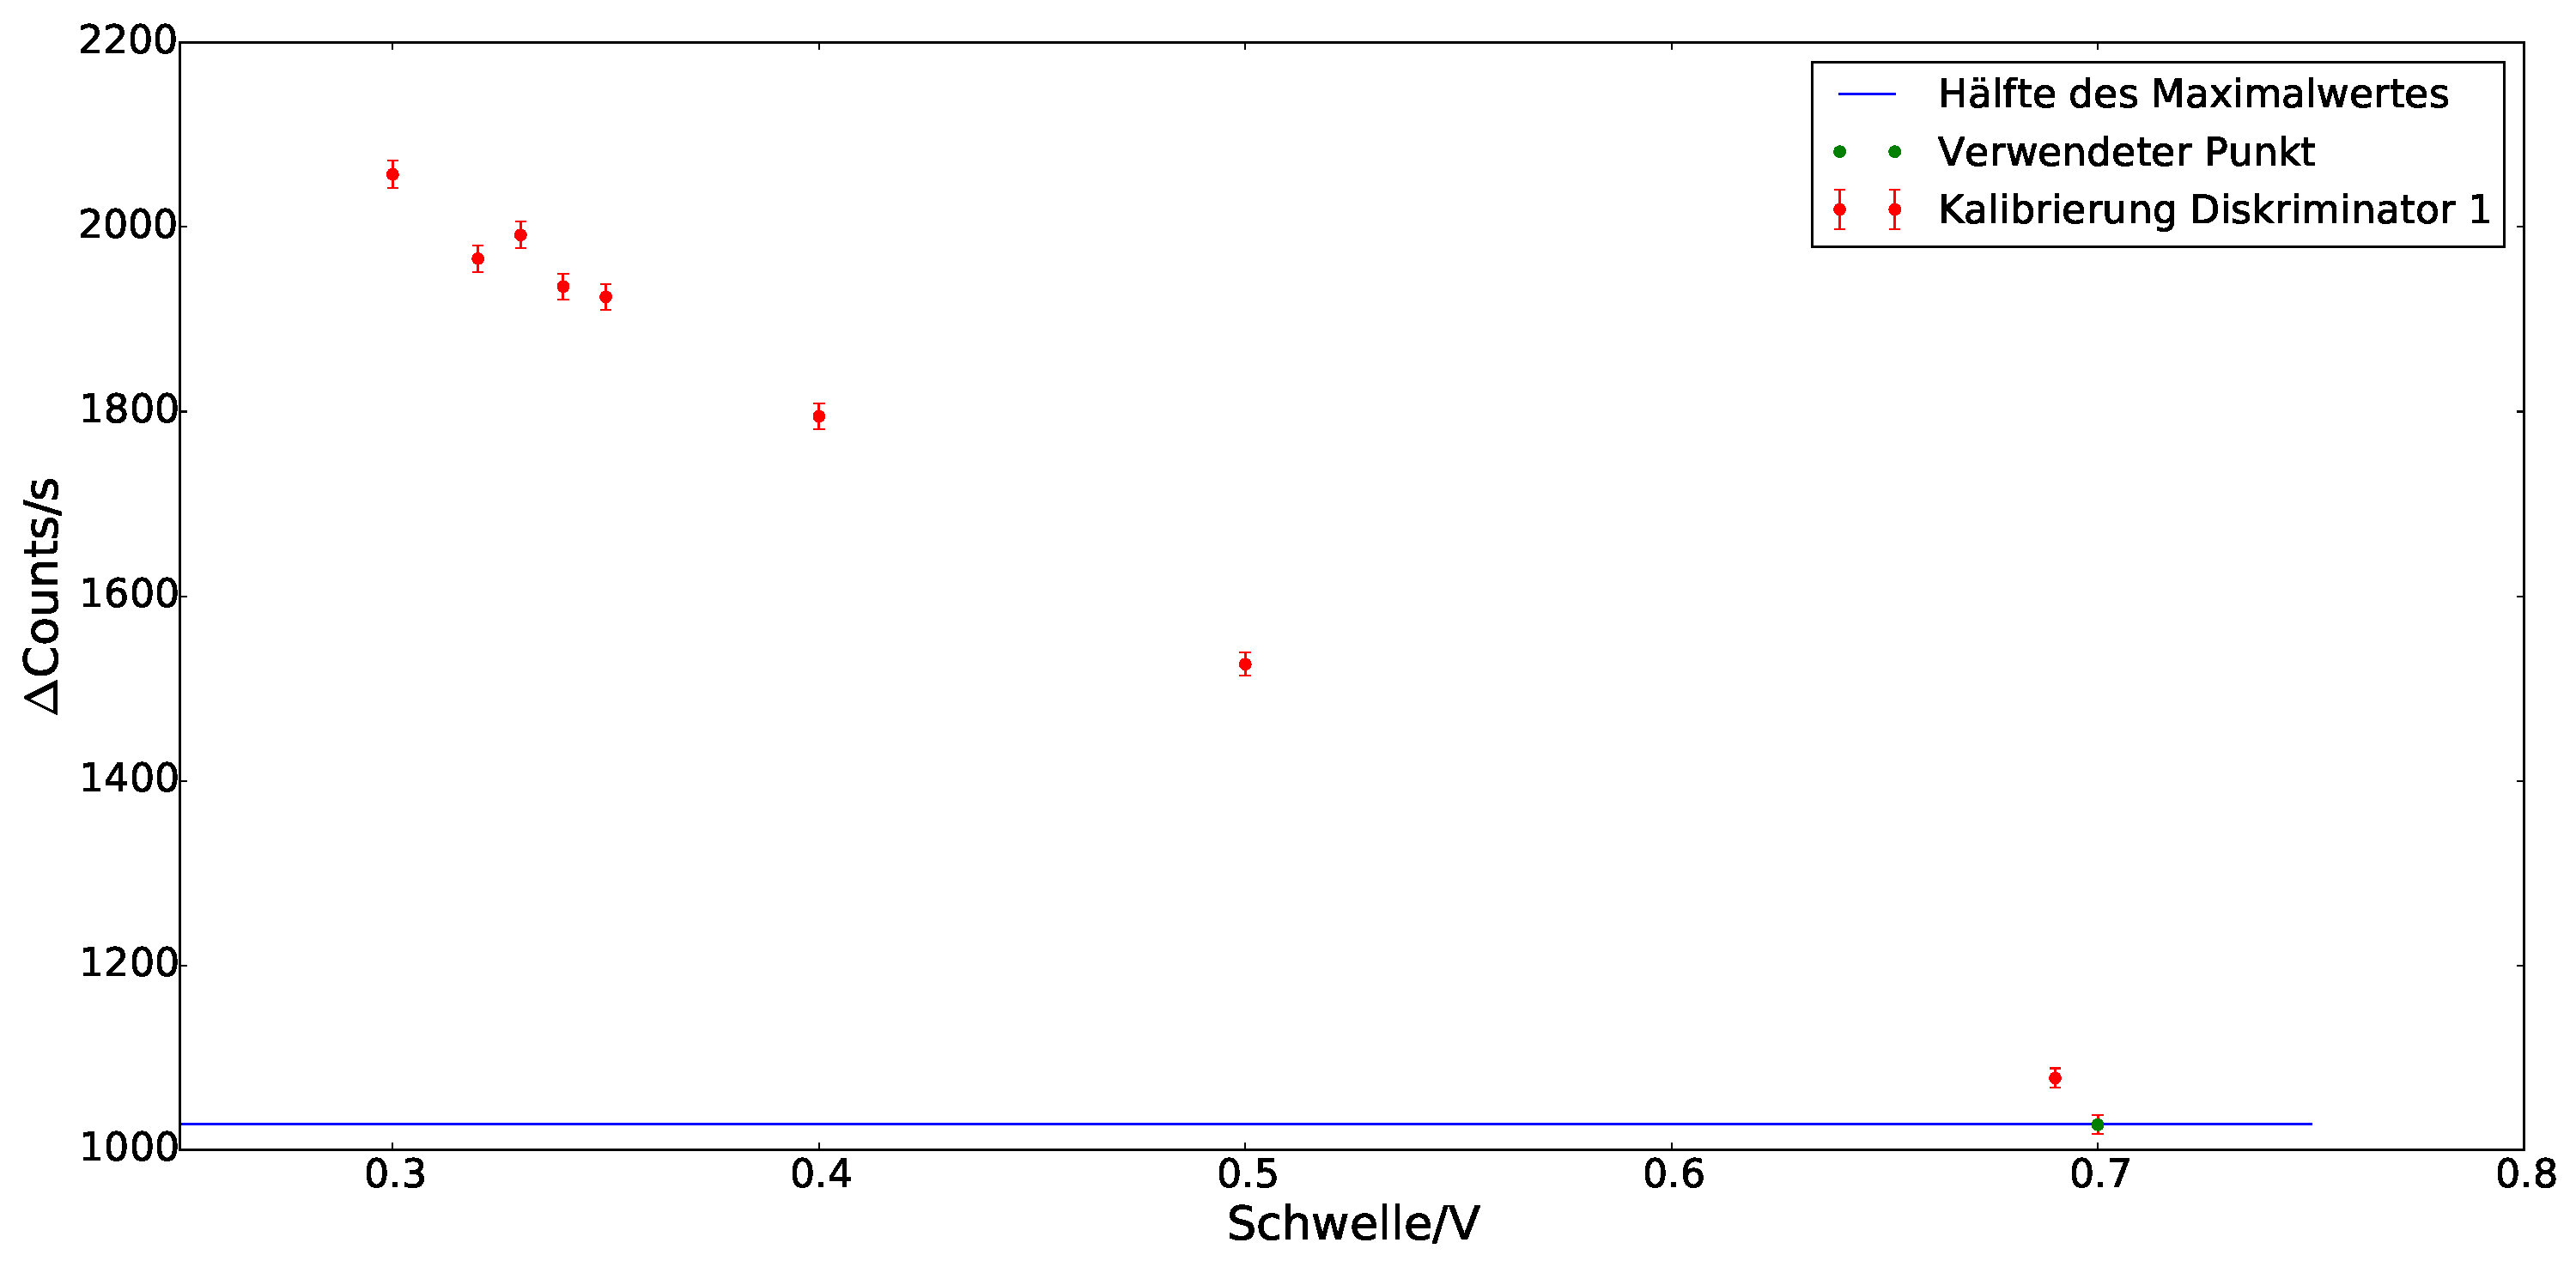
\includegraphics[scale = 0.35]{Disk_1.pdf}
\caption{Differenzplot der Counts gegen die Schwellspannung f�r Diskriminator 1}
\label{fig:Disk_1}
\end{figure}
\begin{figure}[H]
\centering
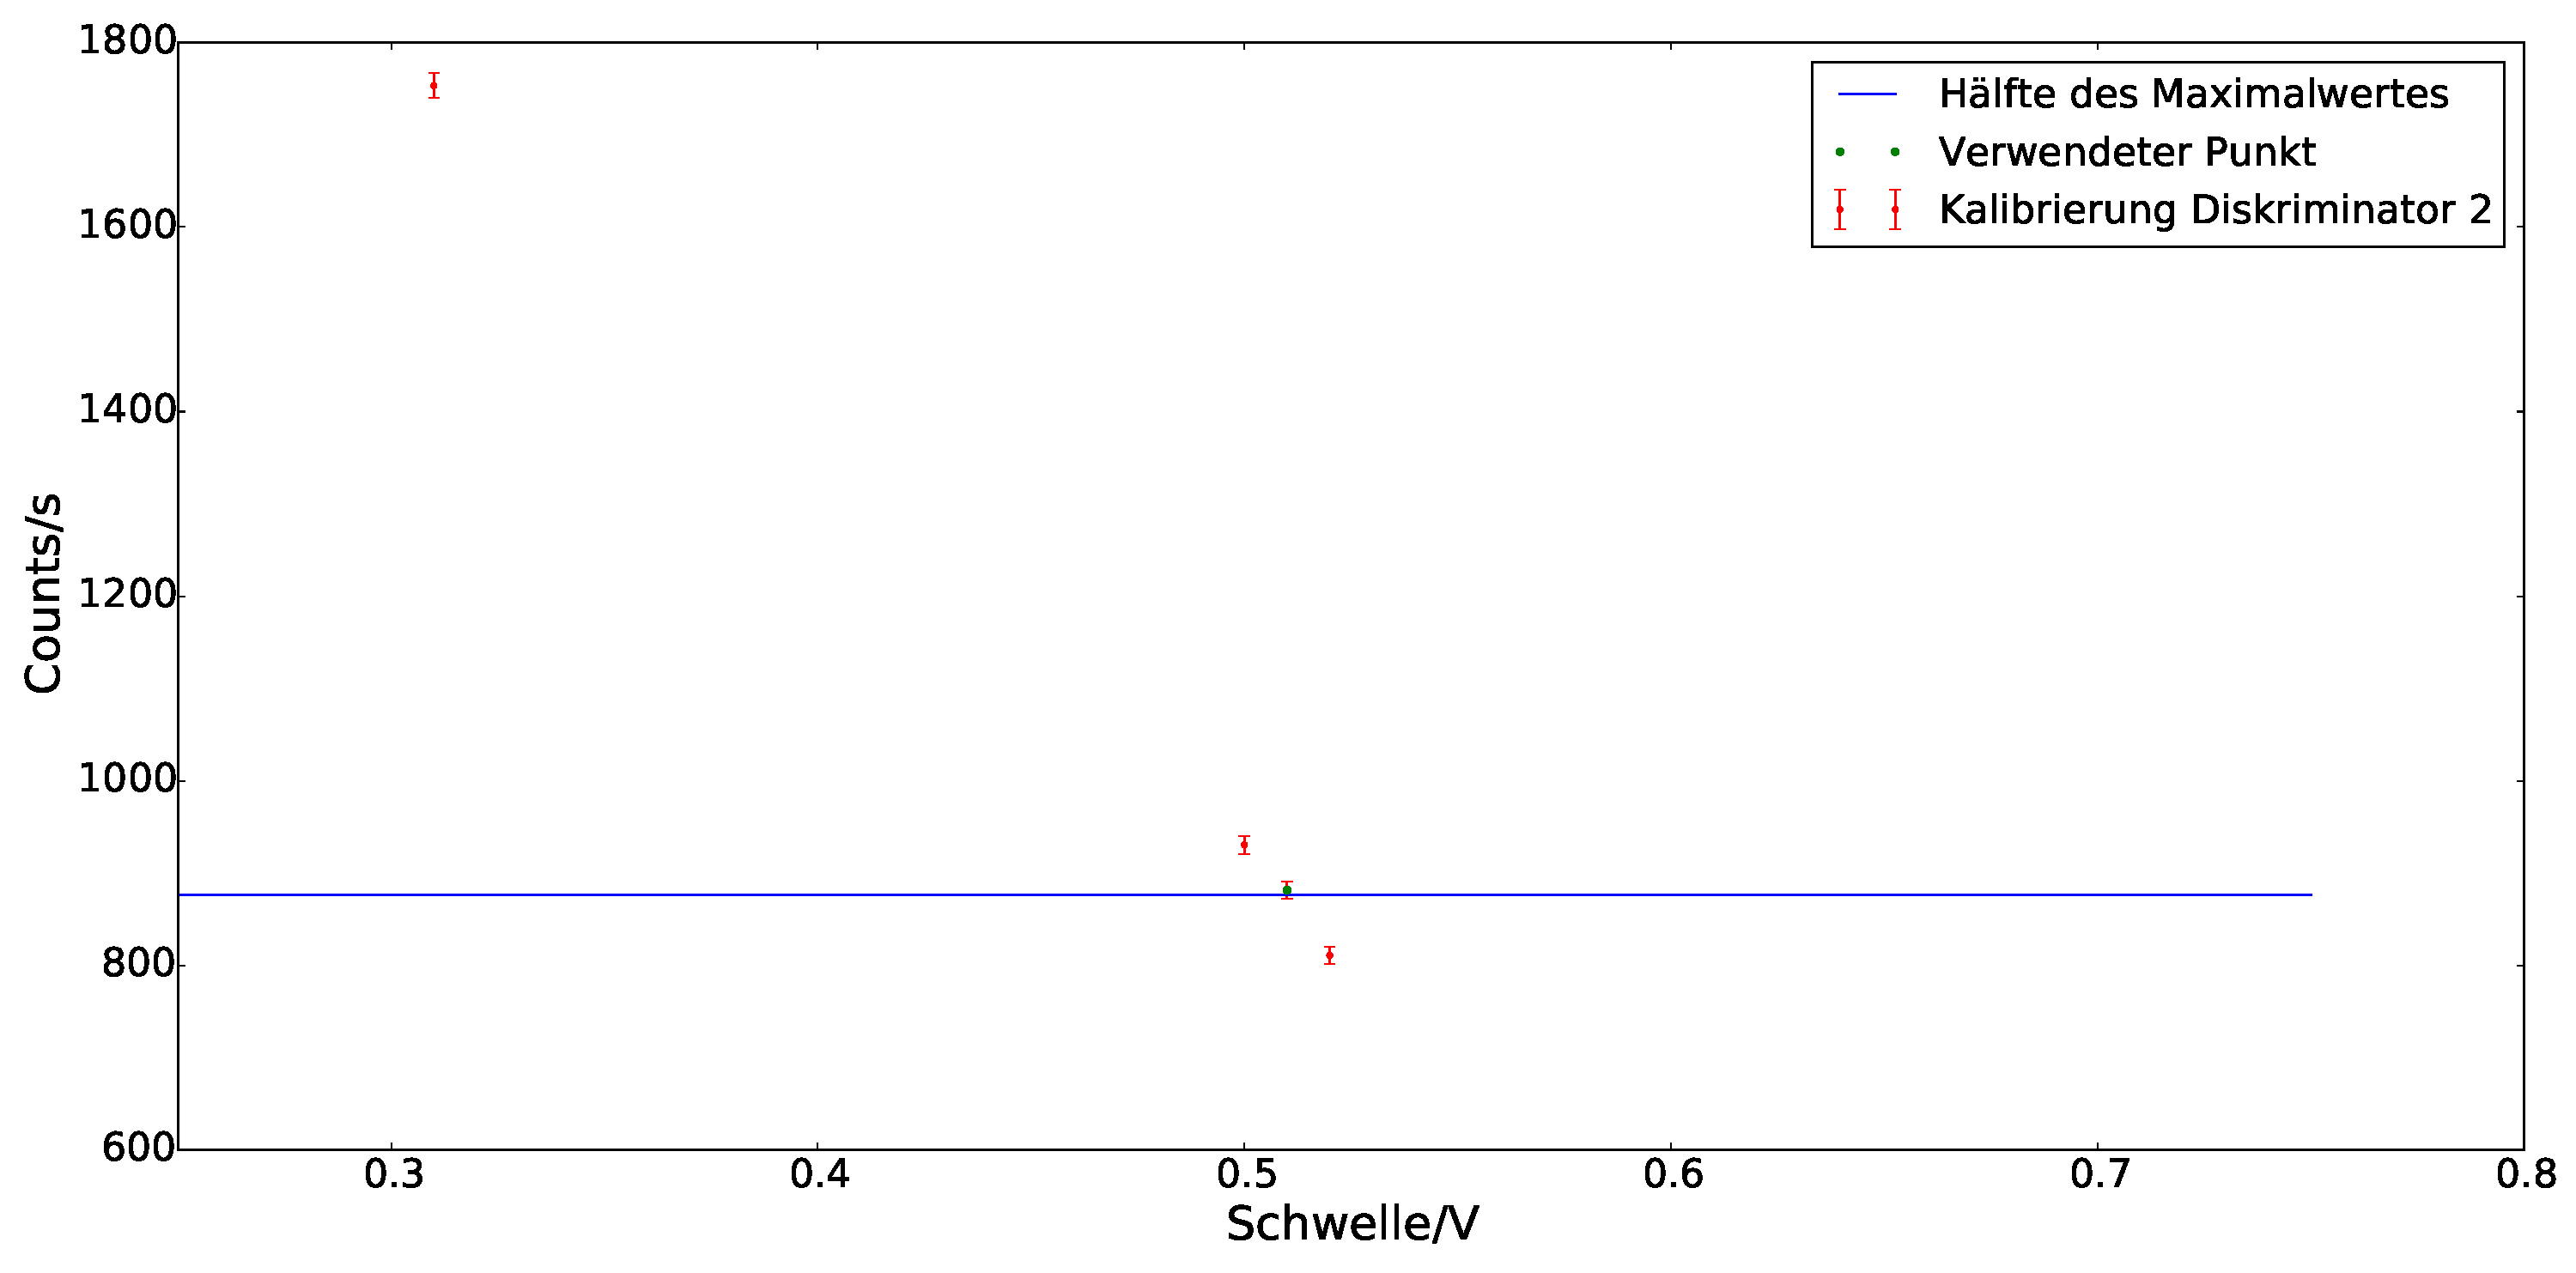
\includegraphics[scale = 0.35]{Disk_2.pdf}
\caption{Differenzplot der Counts gegen die Schwellspannung f�r Diskriminator 2}
\label{fig:Disk_2}
\end{figure}
In Abb. \ref{fig:Disk_3} wurde zus�tzlich eine etwas h�here Schwelle eingestellt, welche auf H�he des Plateaus zwischen den beiden Energien der von $^{60}$Co emittierten Photonen liegt. Nach der Einstellung des Delays, wodurch erreicht werden soll, dass die beiden oberen Szintillatoren (1 und 2) gleichzeitig mit dem 3. Szitillator triggern, wird die Diskriminatorschwelle f�r den 3. Szintillator auf den h�heren Wert gestellt, sodass dieser w�hrend der Messung nur bei Zerfall eines Myons triggert. Szintillator 1 und 2 triggern w�hrend der Messung genau beim Eintritt des Myons in Szintillator 3, wobei Szintillator 3 erst im Falle eines Zerfalls triggert (2. Diskriminatorschwelle). 
\begin{figure}[H]
\centering
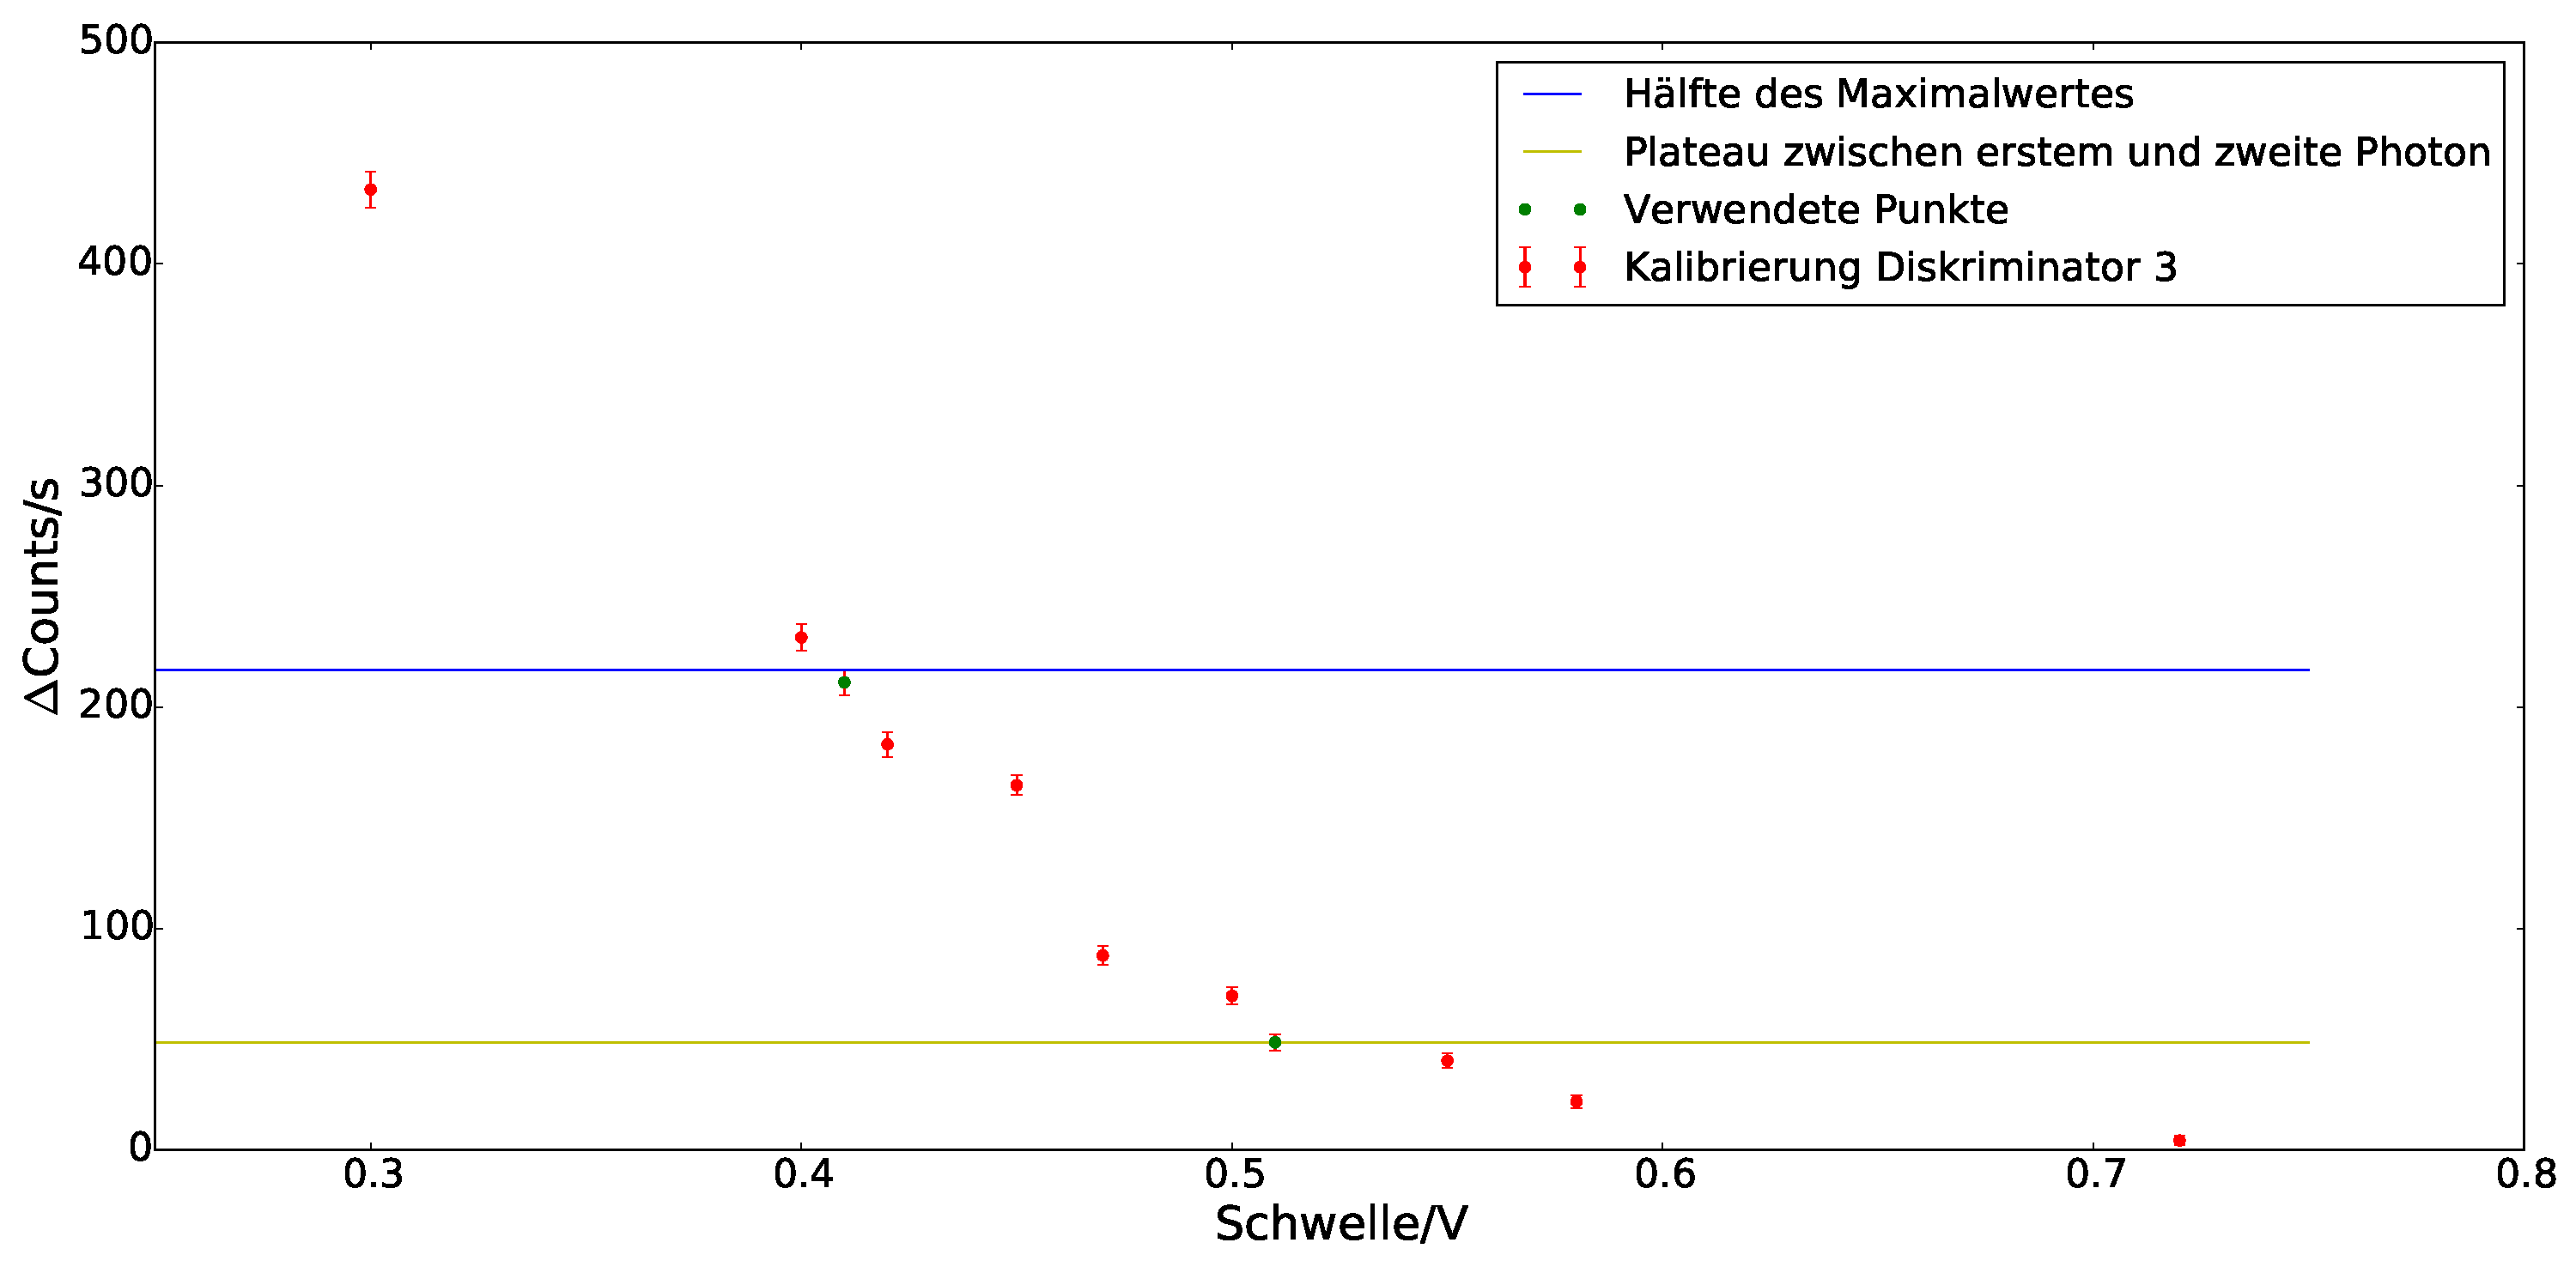
\includegraphics[scale = 0.35]{Disk_3.pdf}
\caption{Differenzplot der Counts gegen die Schwellspannung f�r Diskriminator 3}
\label{fig:Disk_3}
\end{figure}
\begin{figure}[H]
\centering
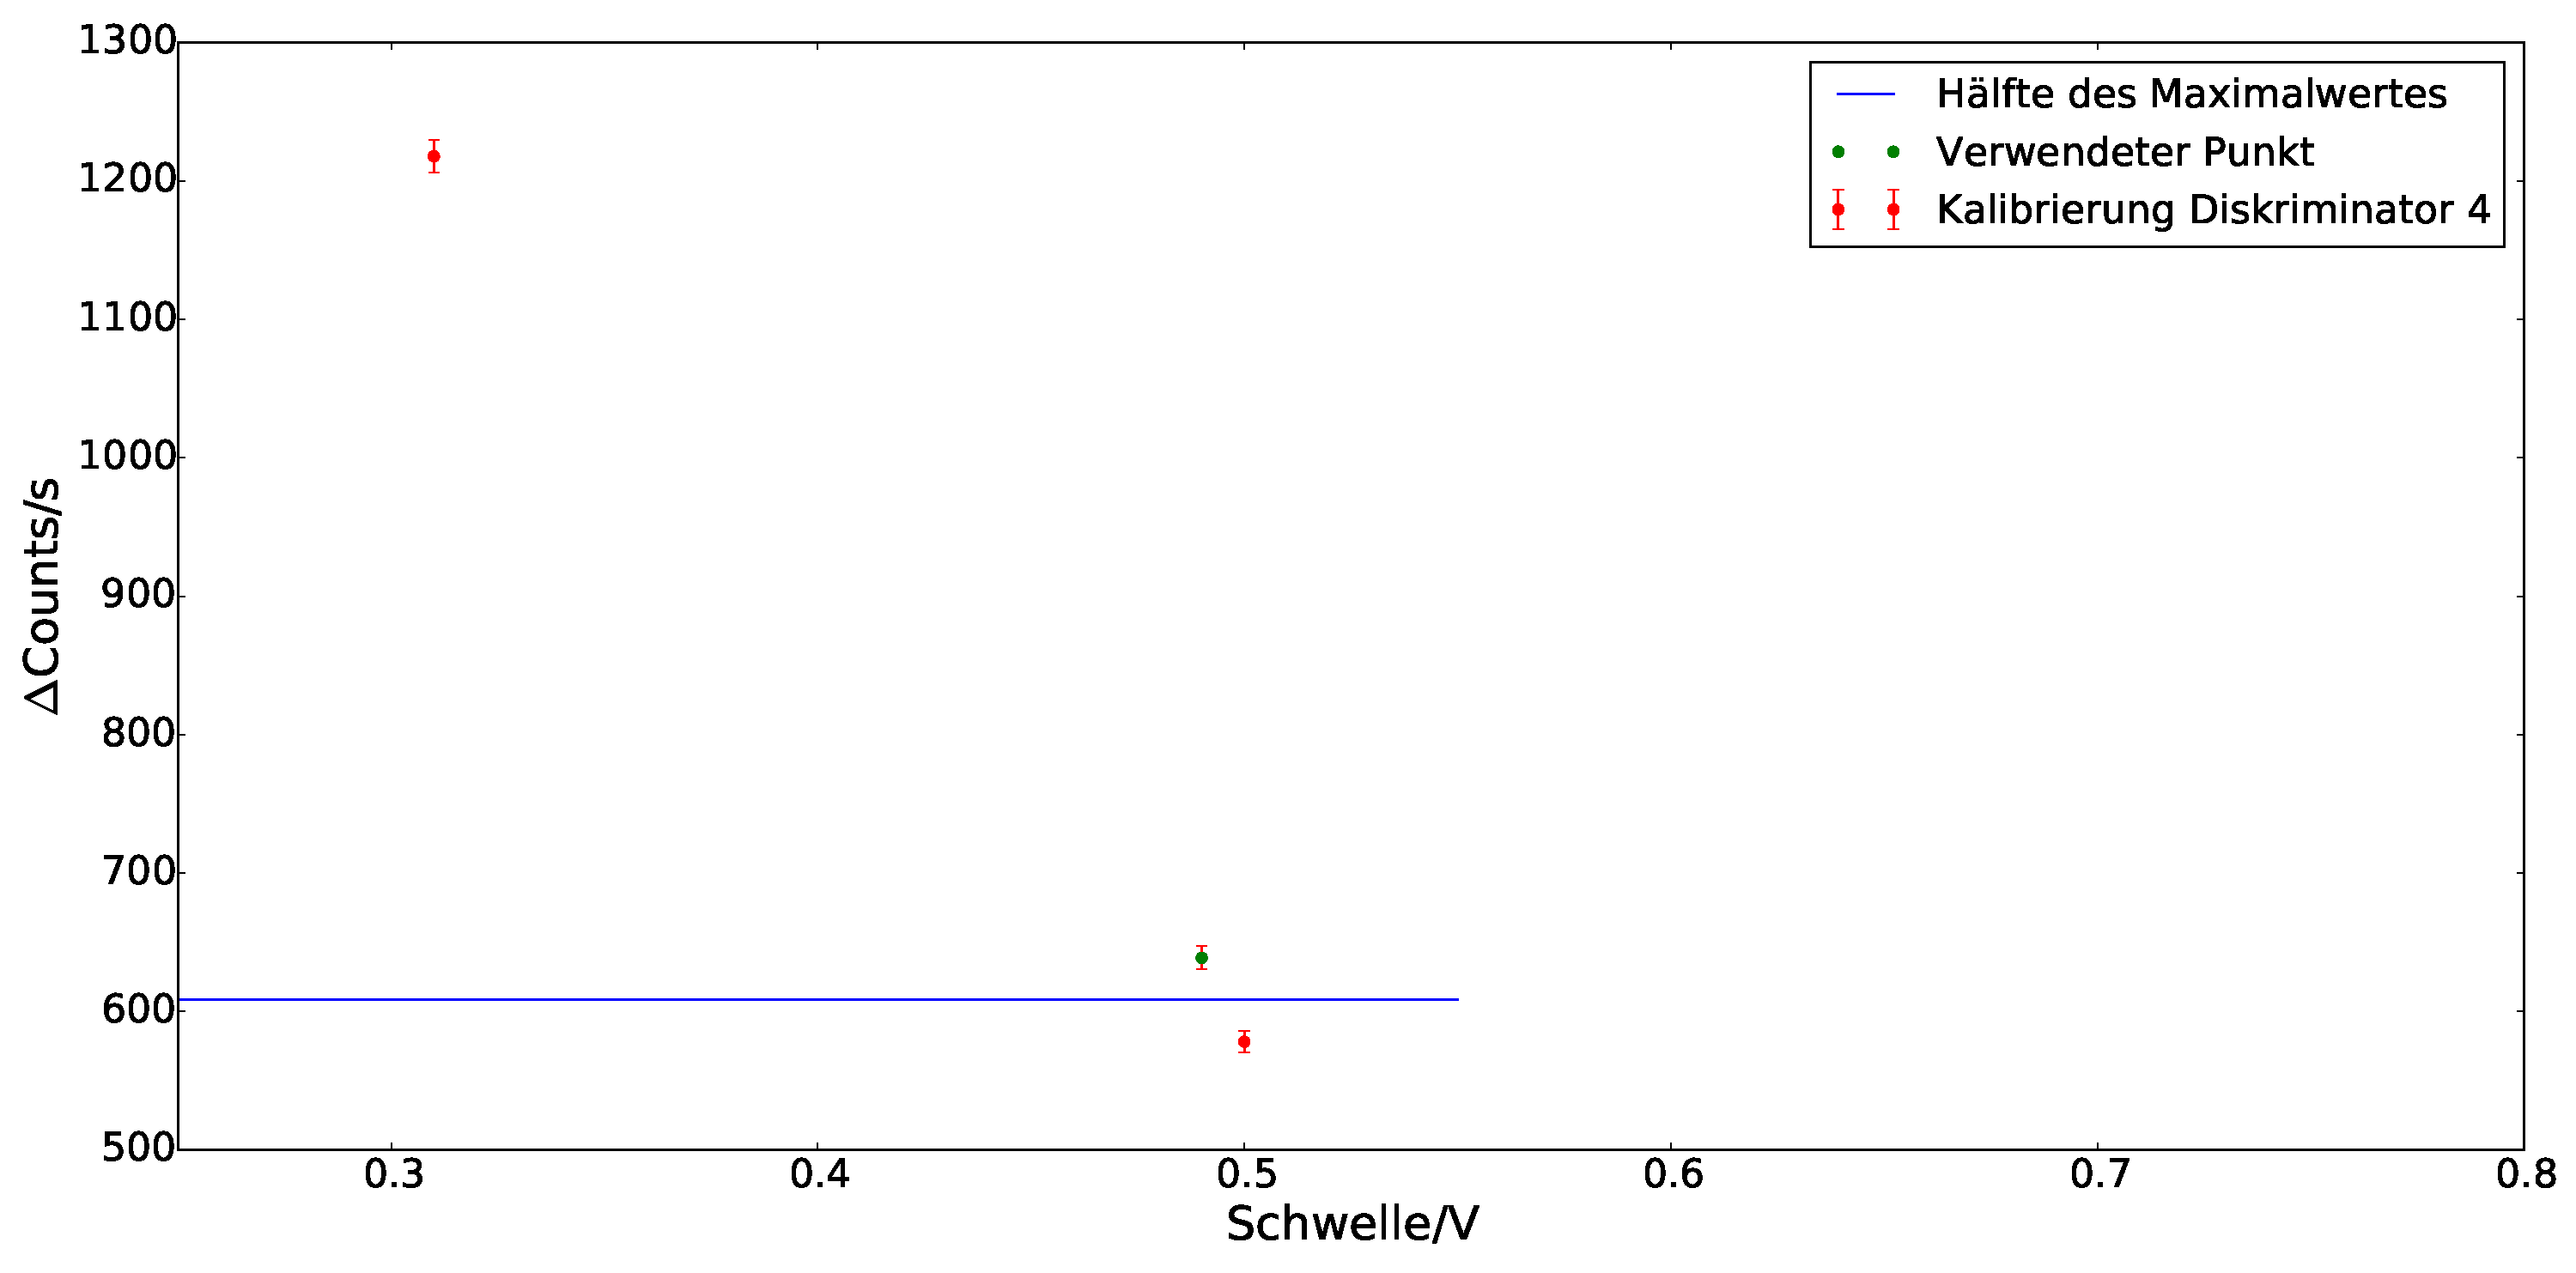
\includegraphics[scale = 0.35]{Disk_4.pdf}
\caption{Differenzplot der Counts gegen die Schwellspannung f�r Diskriminator 4}
\label{fig:Disk_4}
\end{figure}
Die Energien der Photonen beim Zerfall von $^{60}$Co werden in Abb. \ref{fig:Co_60} dargestellt.(vgl. \cite{Co_60})
\begin{figure}[H]
\centering
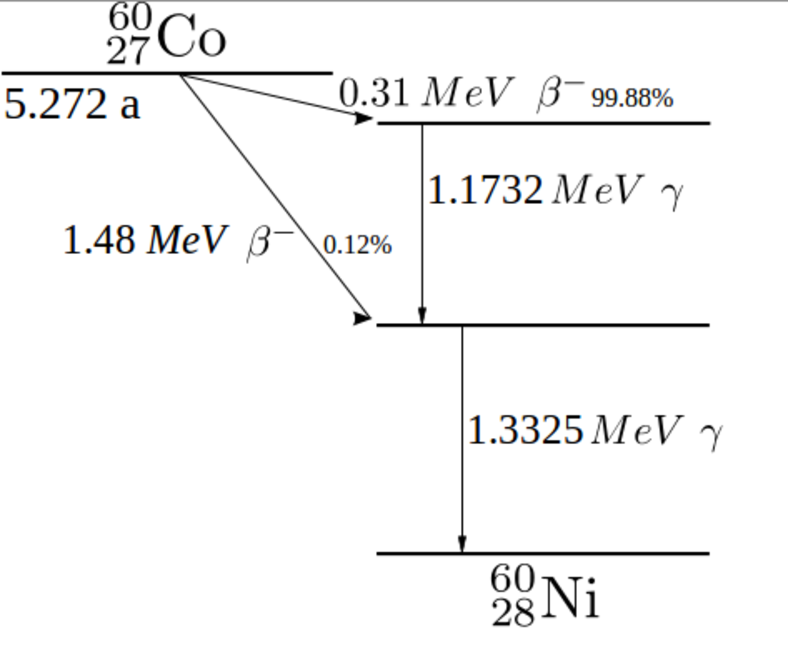
\includegraphics[trim = 0cm 0cm 0cm 1.1nm,scale = 0.5, clip]{Cobalt60_Zerfall.pdf}
\caption{Zerfall von $^{60}$Co}
\label{fig:Co_60}
\end{figure}
In Tabelle \ref{tab:Schwellwerte} sind die Diskriminatorschwellen f�r Diskriminator 1 bis 4 aufgelistet.
\begin{table}[H]
\caption{Diskriminatorschwellwerte}
\begin{tabular}{c|c|c|c|c|}
 & Diskriminator 1 & Diskriminator 2 & Diskriminator 3 & Diskriminator 4 \\ 
\hline Untere Schwelle & 0,70 V & 0,51 V & 0,41 V & 0,49 V \\ 
\hline Obere Schwelle &  &  & 0,52 V &  \\ 
\hline 
\end{tabular}
\label{tab:Schwellwerte}
\end{table}
\subsection{Delay}
Da PM1, PM2 und PM4 �ber eine logische Einheit verbunden sind, welche den TAC startet, muss sichergestellt werden, dass die Signale der drei Photomuliplier Zeitgleich ankommen. Die Zeitversetzung (Delay) der Signale wird �ber die Kabell�nge der Photomuliplier zur logischen Einheit eingestellt.

Es kann angenommen werden, das die Signale von PM3 und PM4 zur selben Zeit ankommen. Deshalb kann das Signal von PM3 gut als Referenz f�r die ersten beiden verwendet werden. F�r die Bestimmung des Delays werden PM1 (bzw. PM2) und PM3 an die logische Einheit angeschlossen, jedoch ohne ein Veto. Die Szintillatoren werden so geschaltet, dass nur bei gleichzeitigem Signal hochgez�hlt wird. Es wird erwartet, das sich ein Plateau ausbildet. Der Delay in der Mitte des Plateaus ist die optimale Einstellung, das sich die Signale an diesem Punkt �berlagern. Damit sich ein m�glichst schmales Plateau ausbildet, m�ssen die Pulse der Diskriminatoren kurz sein. In Abbildung \ref{fig:delay_1} ist zu sehen, dass f�r den ersten Photomulipier kein eindeutiges Plateau identifiziert werden konnte. Deshalb musste das Delay mit dem Oszilloskop eingestellt werden, um sicherzustellen, dass sich die beiden Signale �berlappen. F�r den ersten Photomuliplier wurde mit dem Oszilloskop ein Delay von 9ns bestimmt. In Abbildung \ref{fig:delay_2} sind die Messdaten f�r den zweiten Photomuliplier zu sehen. Im Bereich von 20 bis 28ns ist ein Plateau zu erkennen, das Delay wurde mit dem Wert (24ns) in der Mitte des Plateaus angenommen. Das Delay von 24ns f�r den zweiten Photomuliplier wurde zus�tzlich mit dem Oszilloskop bestimmt und konnte best�tigt werden.

\begin{figure}[H]
	\centering
  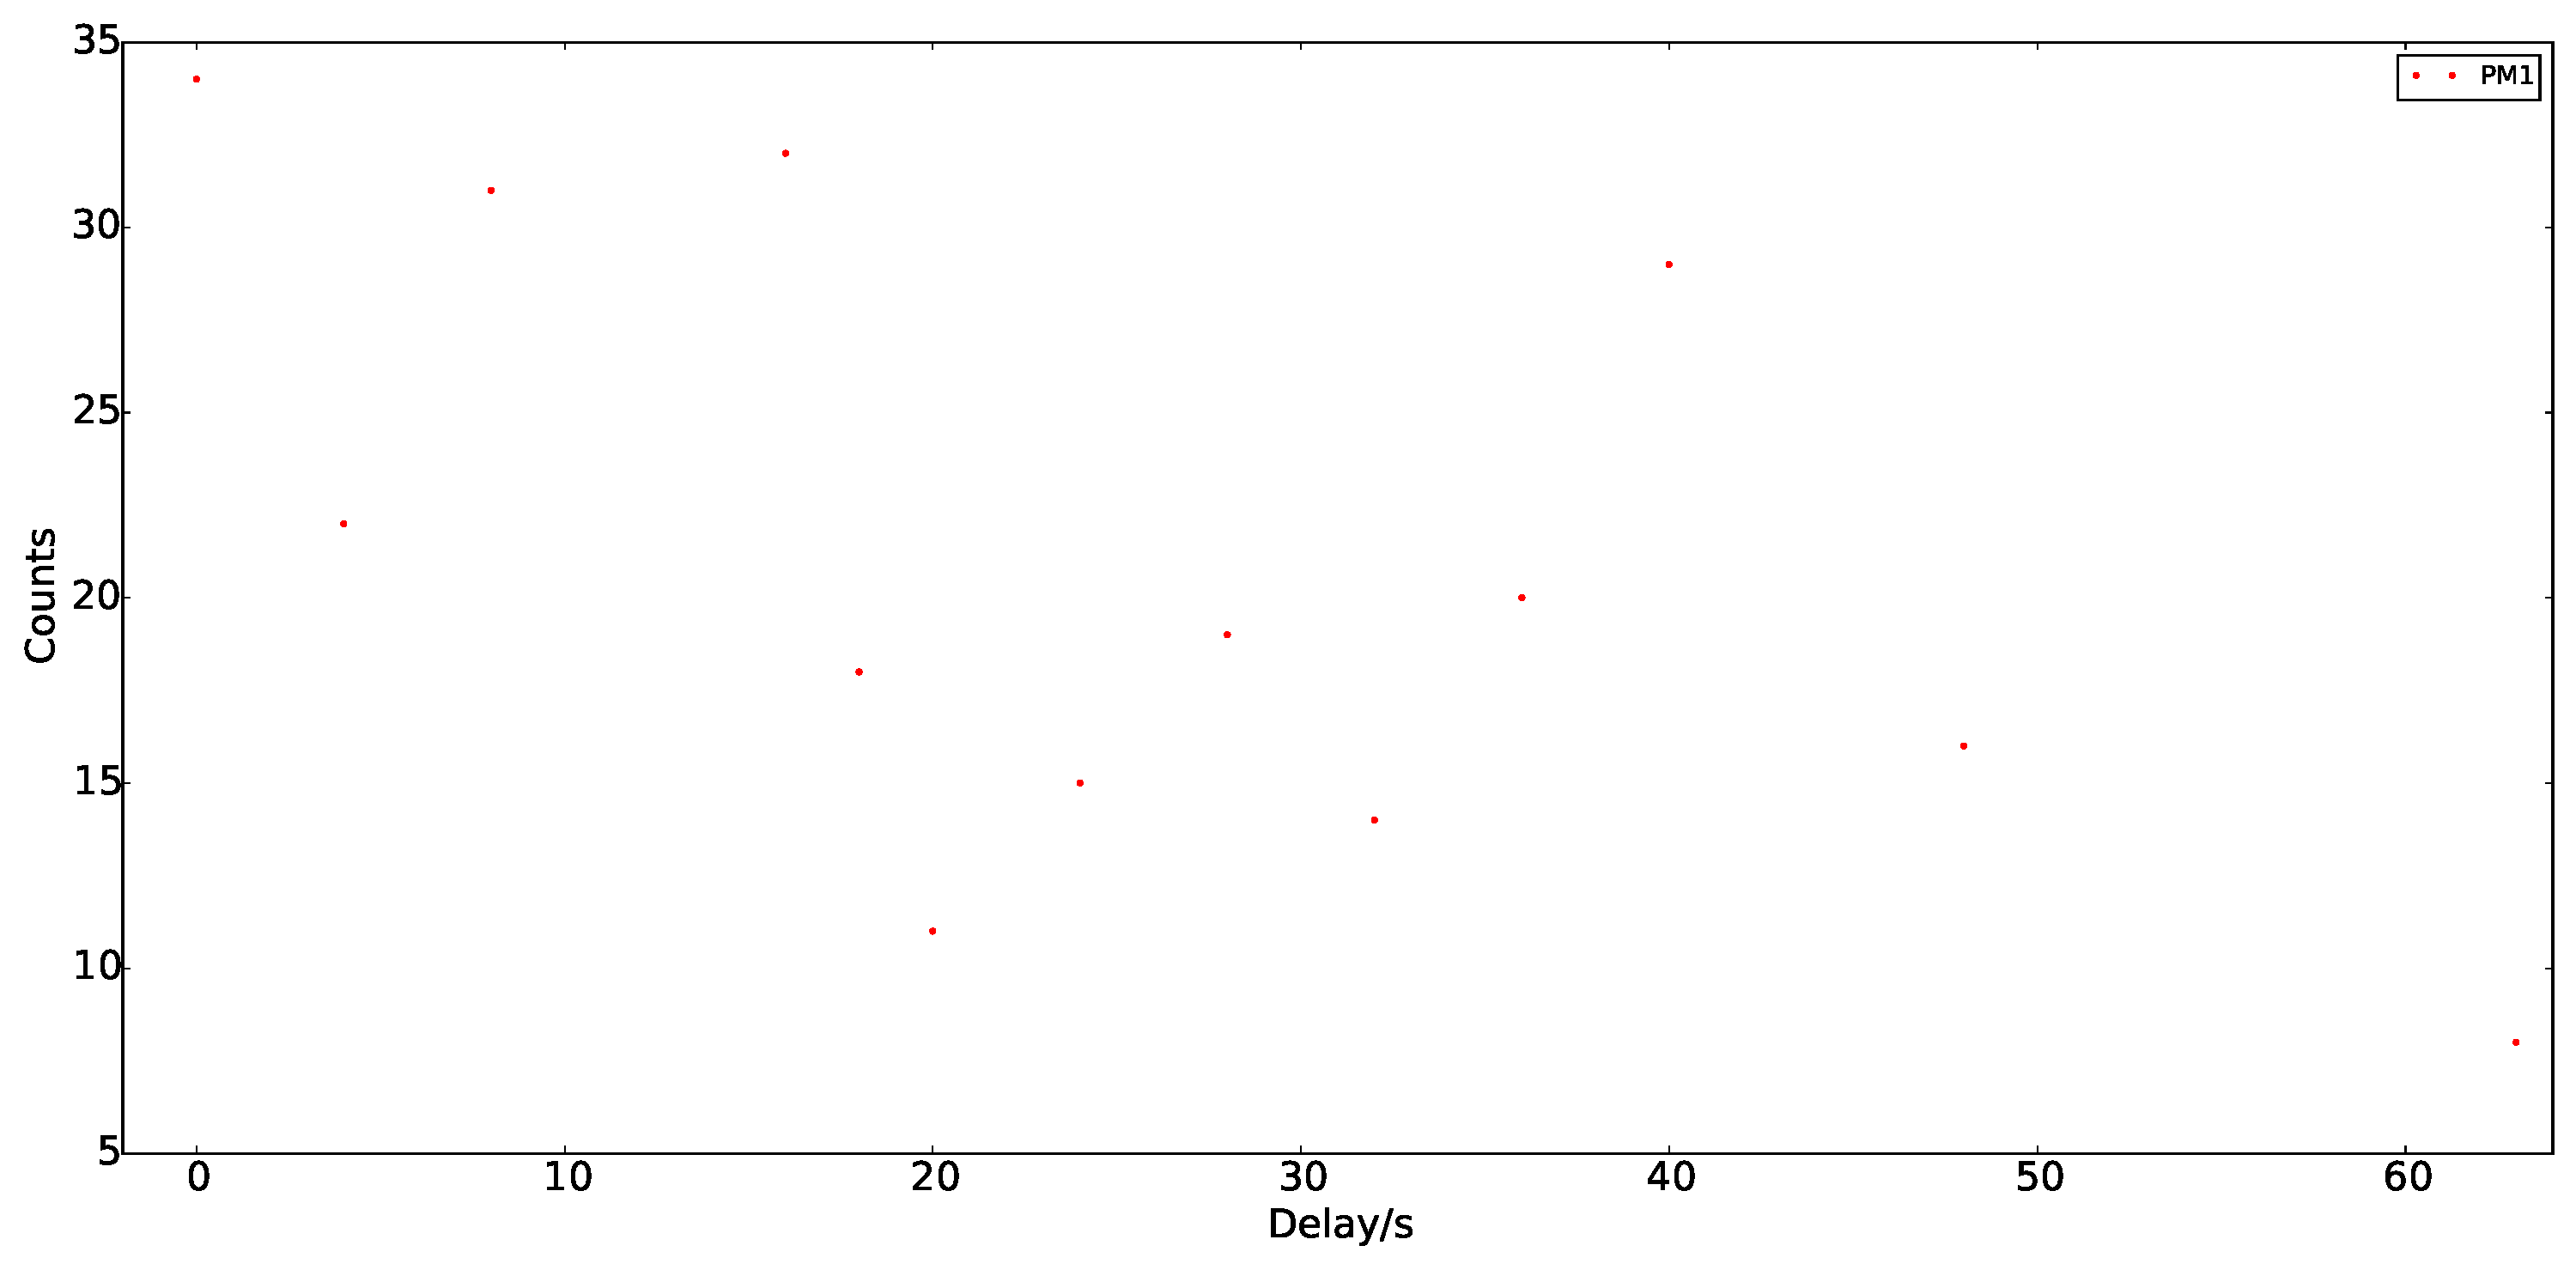
\includegraphics[scale=0.33]{delay_1.pdf}
	\caption{Counts in Abh�ngigkeit vom Delay f�r die ersten Photomuliplier, es ist kein eindeutiges Plateau zu erkennen. Deshalb wurde das Signal mit einem Oszilloskop betrachtet und ein Delay von 9ns bestimmt.}
	\label{fig:delay_1}
\end{figure}


\begin{figure}[H]
	\centering
  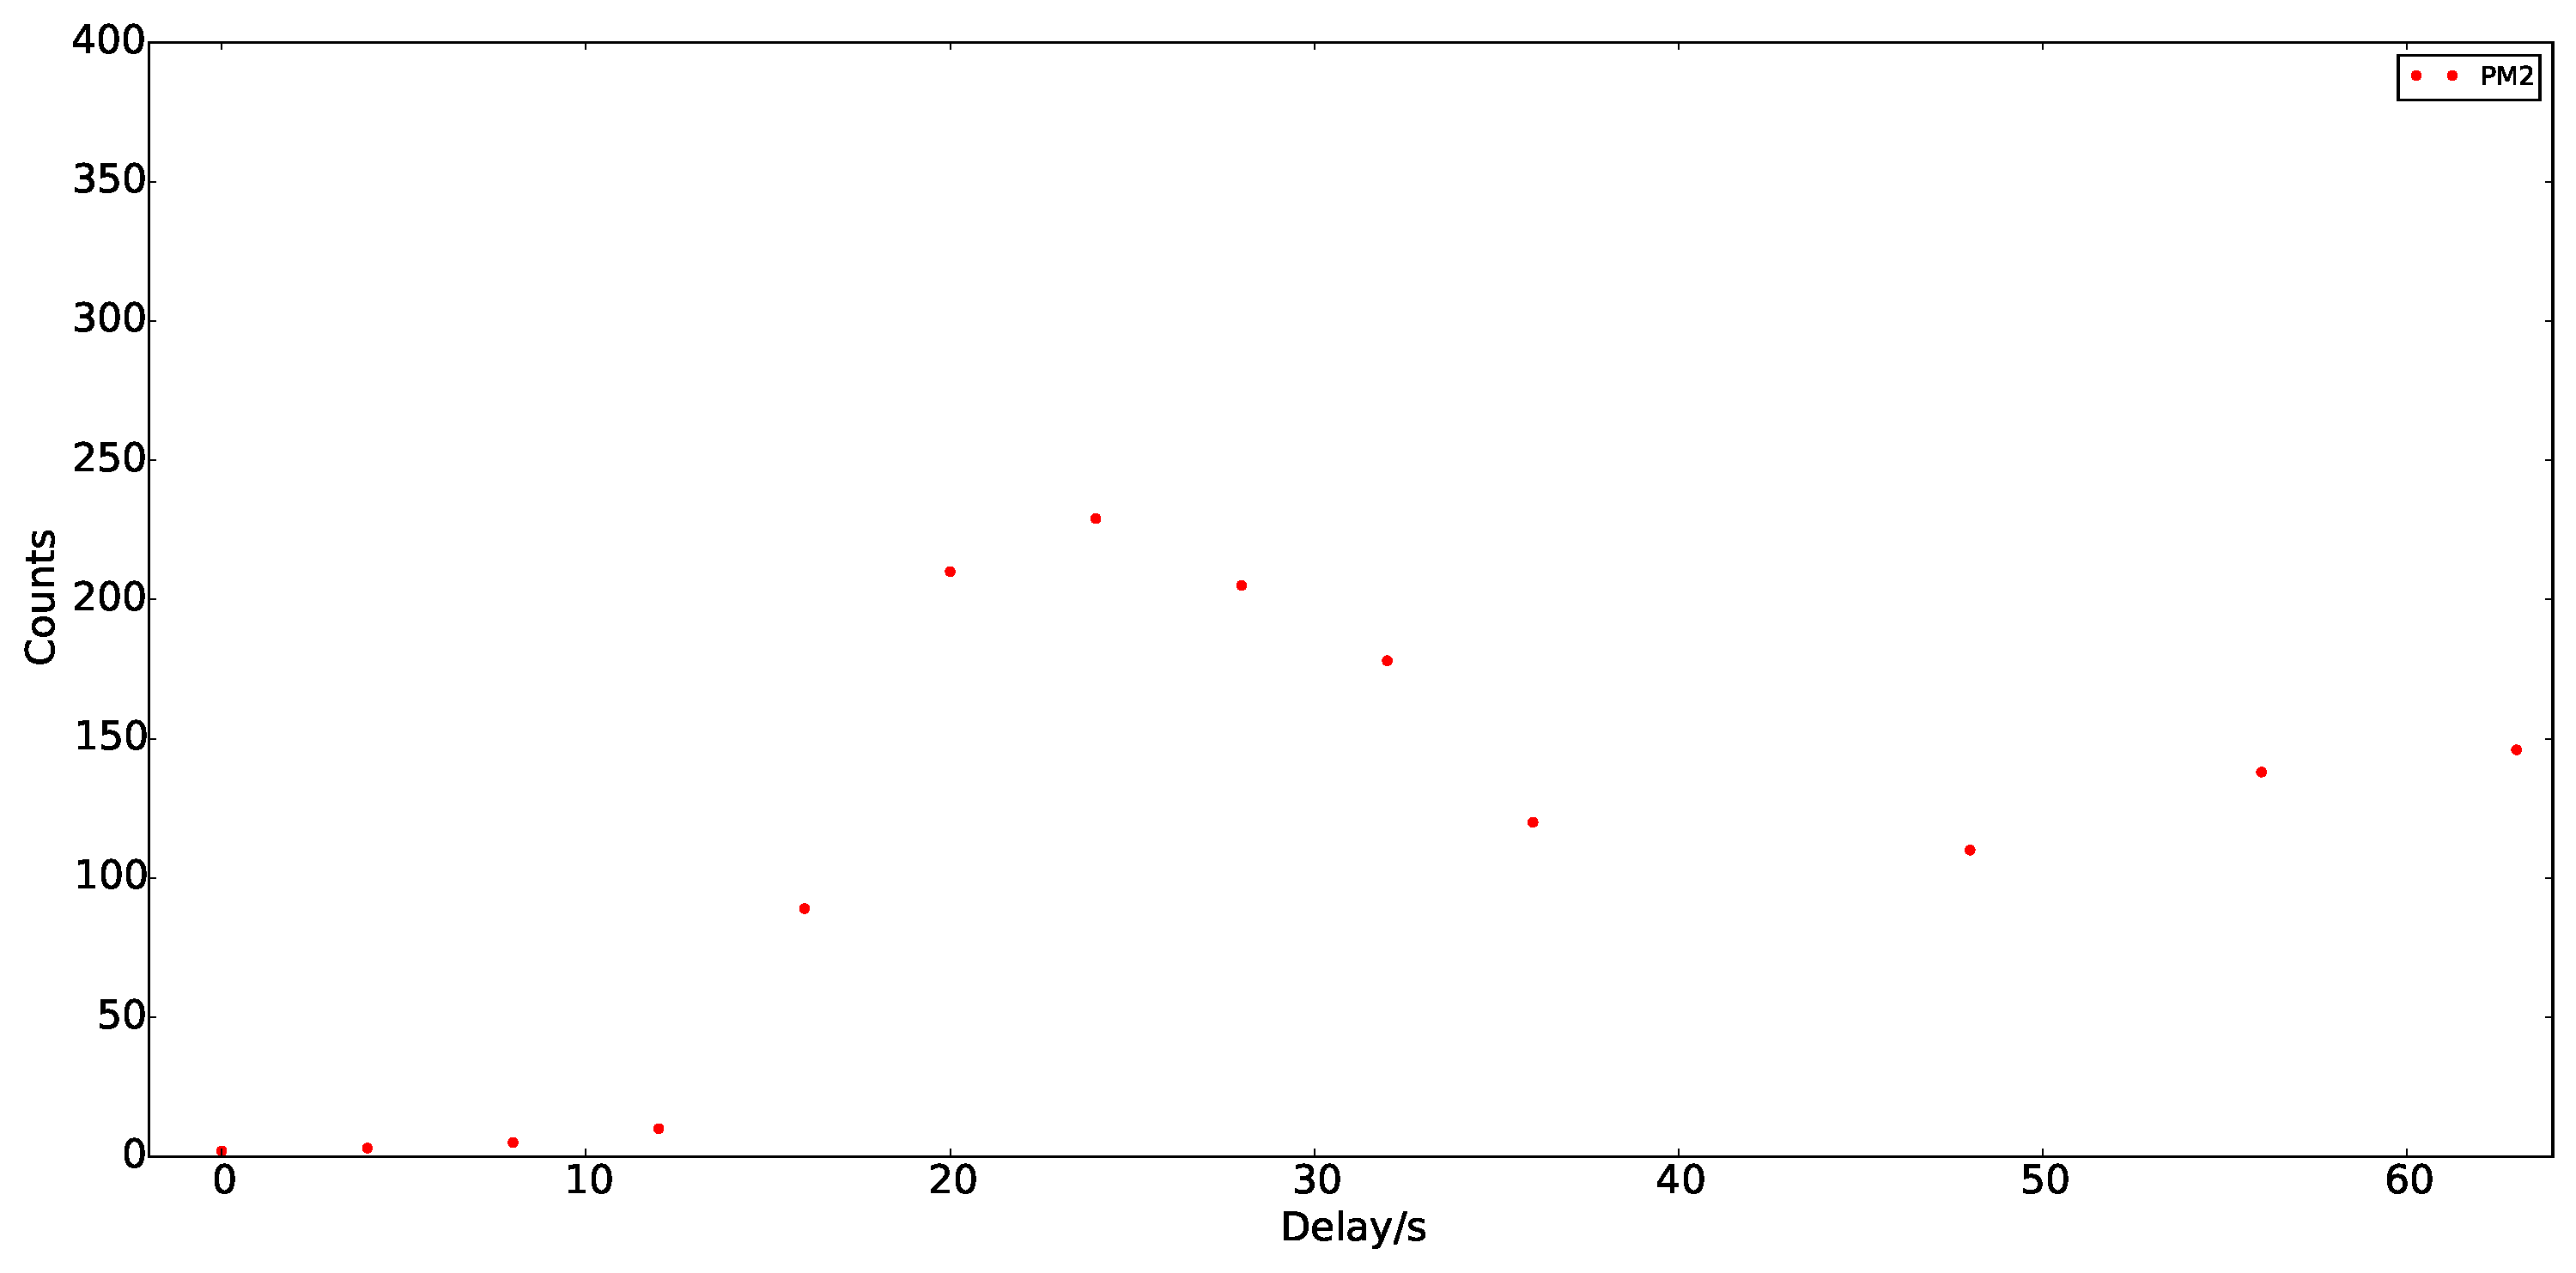
\includegraphics[scale=0.33]{delay_2.pdf}
		\caption{Counts in Abh�ngigkeit vom Delay f�r die ersten Photomuliplier. Ein Plateau ist im Bereich von 20 bis 28 ns zu erkennen. Das Delay wurde mit 24 ns, in der Mitte des Plateaus bestimmt. dieser Wert wurde mit dem Oszilloskop verifiziert.}
	\label{fig:delay_2}
\end{figure}

Es ergeben sich die Delays in Tabelle \ref{tab:delay}.

\begin{table}[H]
	\centering
	\caption{Optimal bestimmtes Delay f�r PM1 und PM2}
	\label{tab:delay}
	\begin{tabular}{|c|c|}
	\hline Photomuliplier & Delay [ns] \\ \hline
	\hline PM1 & 9 \\ 
	\hline PM2 & 24 \\ 
	\hline 
	\end{tabular} 
\end{table}

Das Oszilloskopbild Abb. \ref{PMT2Delay} zeigt, dass die Signale beim zweiten Photomultiplier �bereinander liegen. Auff�llig war, dass trotz Abschlusswiderstand verschobene Signale angezeigt wurden, die eigentlich nicht zu sehen sein sollten.
\begin{figure}[H]
\centering
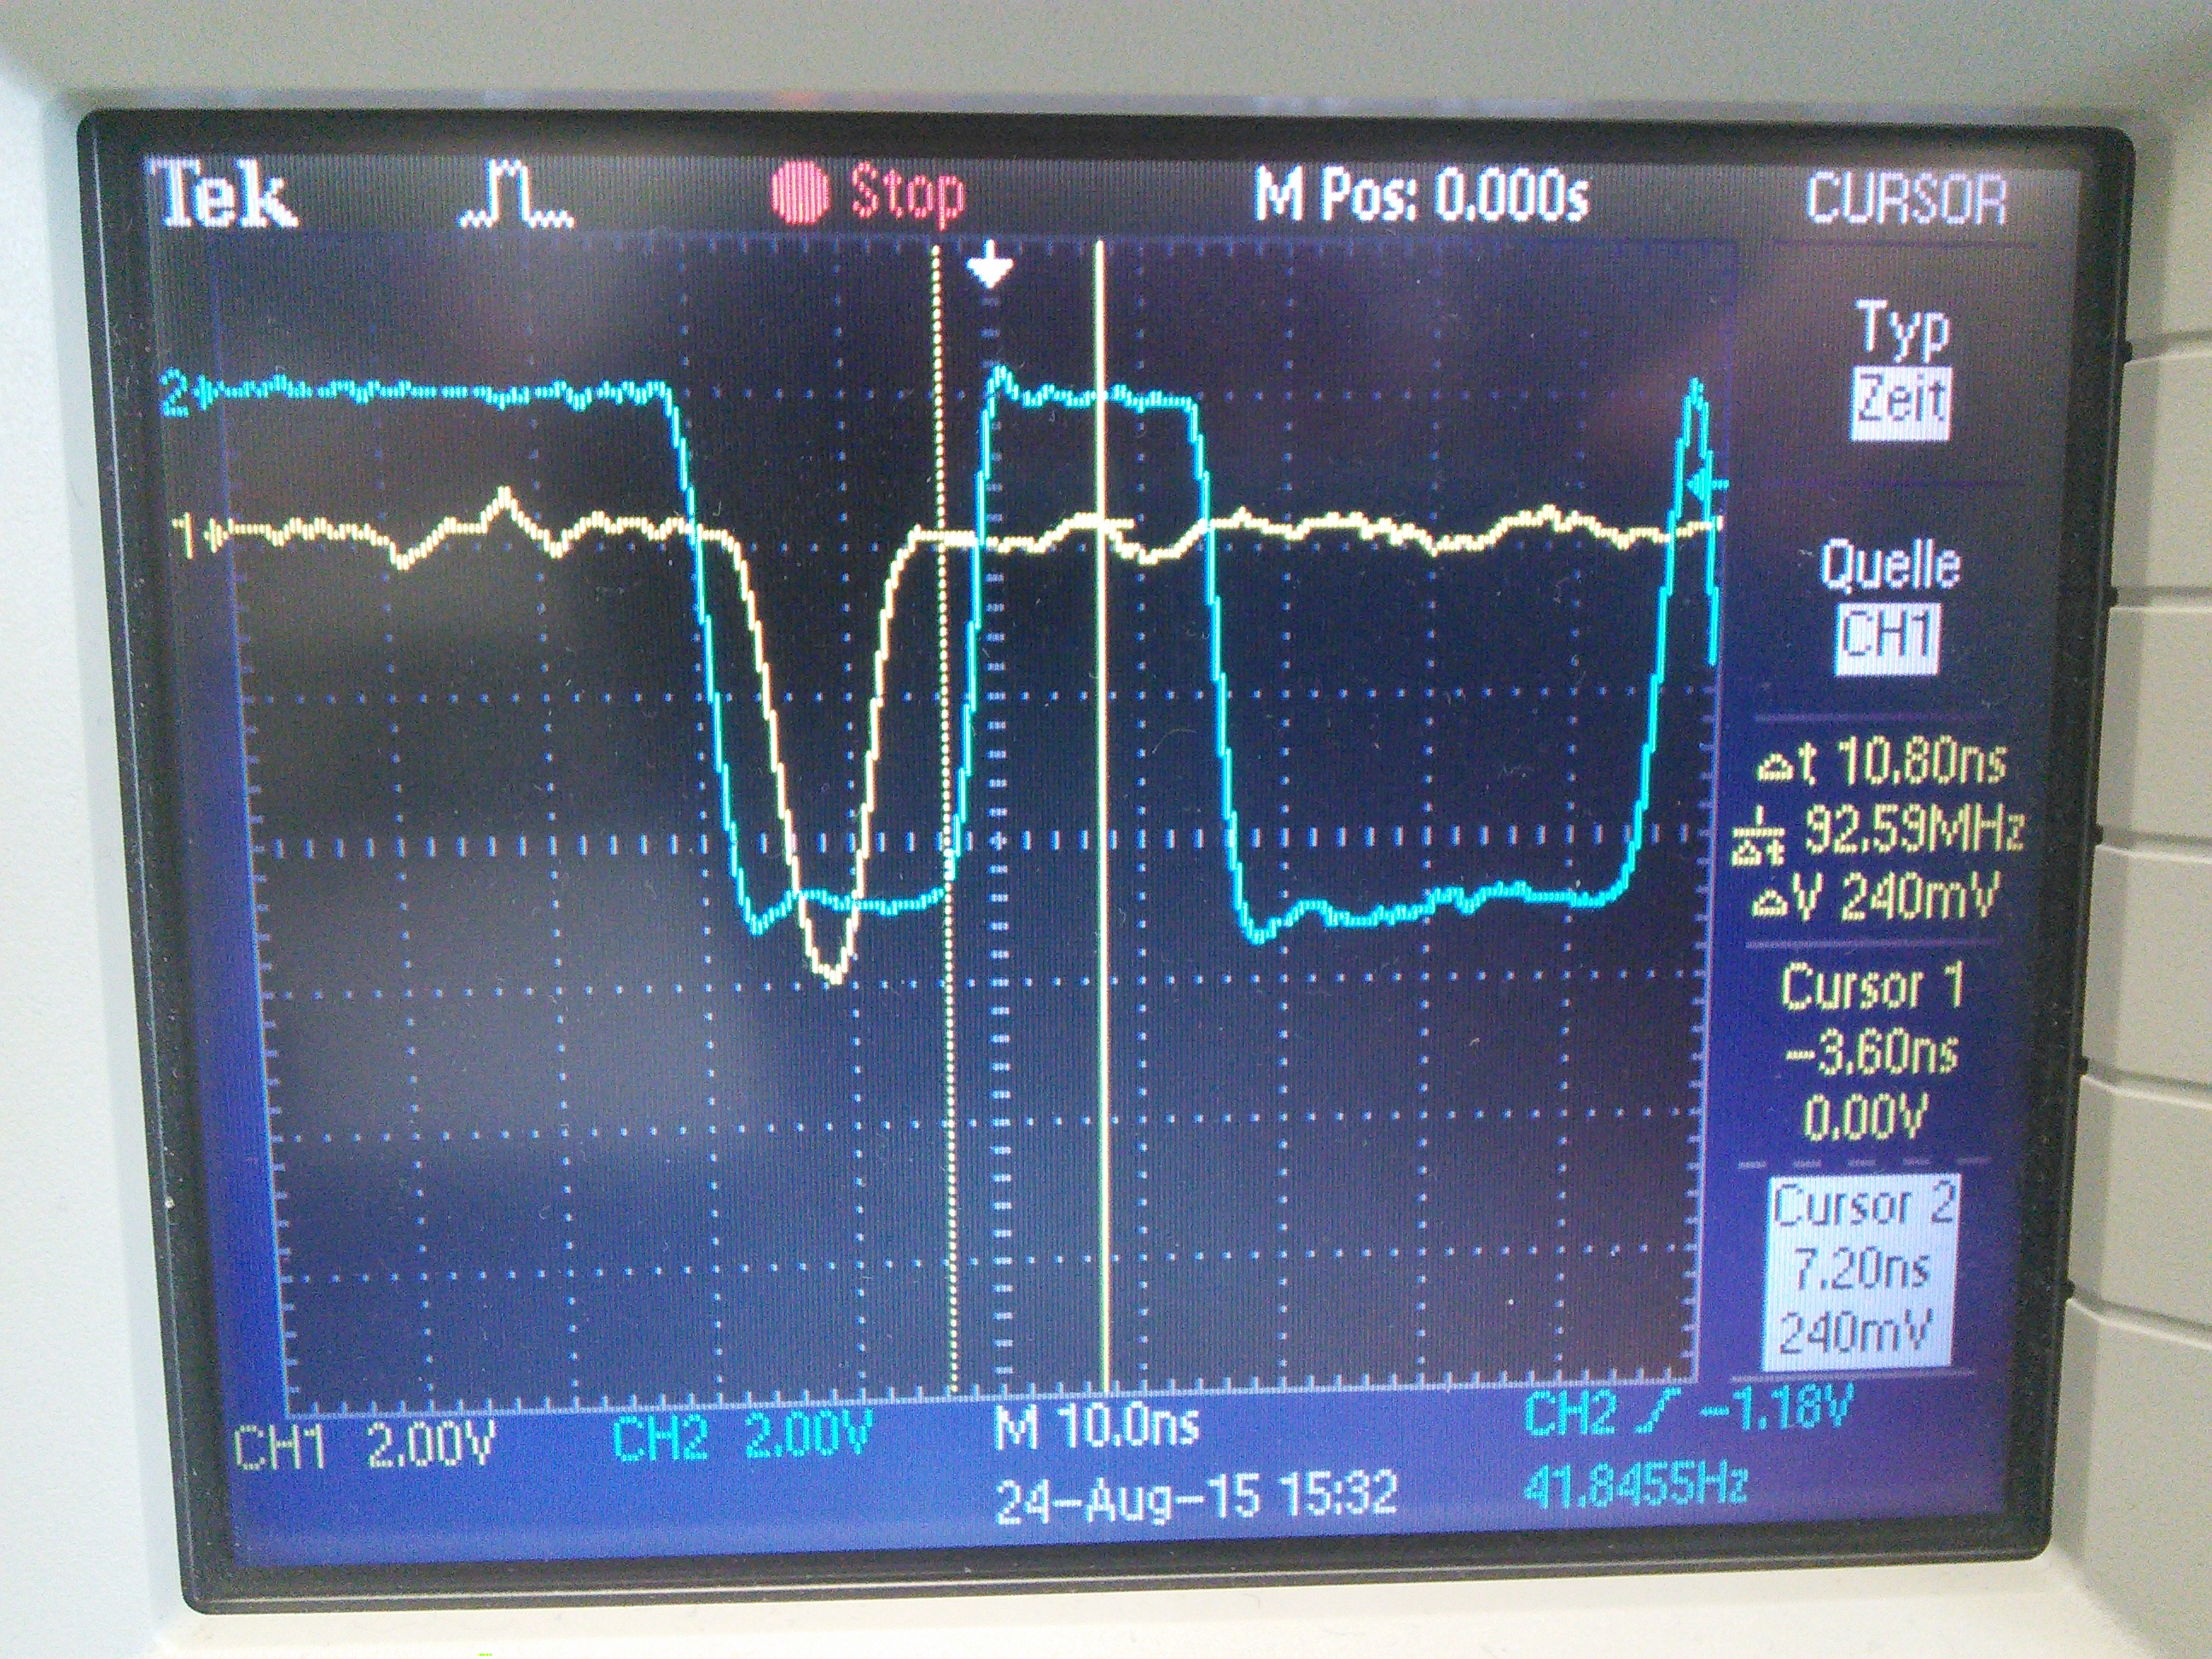
\includegraphics[scale=0.12]{DelayPMT2}
\caption{Oszilloskopbild Delay PMT 2}
\label{PMT2Delay}
\end{figure}
\subsection{Kanal-Zeit-Eichung}
F�r eine genaue Bestimmung der Lebensdauer von Myonen ist eine exakte Zeiteichung extrem wichtig. F�r die Zeiteichung wird ein TAC, ein dual Timer und ein Oszilloskop verwendet. Der schematische Aufbau ist in Abbildung \ref{fig:kanal_zeit} zu sehen. 

\begin{figure}[H] 
	\centering
  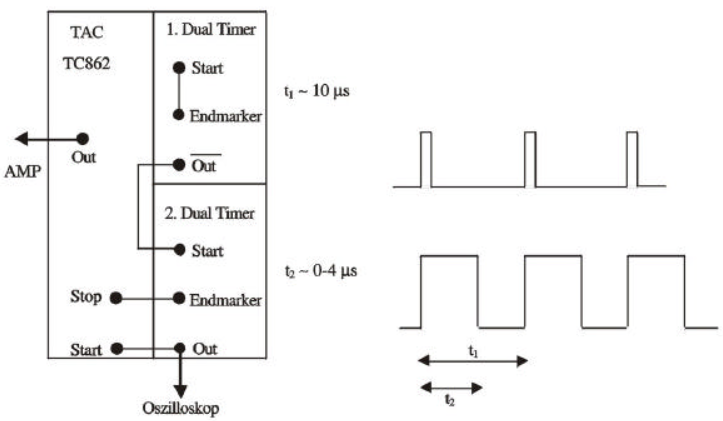
\includegraphics[scale=0.5]{kanal_zeit.png} 
	\caption{Schematischer Aufbau f�r die Kanal-Zeit-Eichung}
	\label{fig:kanal_zeit}
\end{figure}

Der dual Timer wird verwendet, um kurze Signale mit bekannter L�nge zu erzeugen. �ber die High und Lows des Signals wird der TAC gesteuert, wodurch eine Spannung in Abh�ngigkeit der L�nge des Signals erzeugt wird. Das Signal wird verst�rkt und mit dem ADC digitalisiert, damit es vom Mulit-Channel-Analyser verwertet werden kann. Durch variiren der Signall�nge lassen sich die verschiedene Kan�le ansprechen, wodurch eine Beziehung zwischen einer Zeit und einem Kanal hergestellt wird. Die Zeitintervalle werden gegen die Kan�le aufgetragen und mit Gleichung \ref{eqn:kanal} gefittet. Zum Vergleich soll zus�tzlich ein Fit mit $B = 0$ erzwungen werden. Die Parameter und Variablen des Fits sind in Tabelle \ref{tab:fit_kanal} zu sehen

\begin{align}
\label{eqn:kanal}
t = A*k+B
\end{align}

\begin{table}[H]
	\caption{Parameter des Fits}
	\label{tab:fit_kanal}
	\begin{tabular}{c|l}
	t & Zeitintervall in $\mu$s \\ 
	k & Kanal \\ 
	A & Proportionalit�tsfaktor \\ 
	B & Offset \\ 
	\end{tabular} 
\end{table}

In Abbildung \ref{fig:kanal_zeit_fit} sind die Messwerte zu sehen. F�r die Fitparameter ergaben sich dabei die Werte in Tabelle \ref{tab:fit}. Das $\chi_{red}^2$ hat ein Wert von 0,02, was einem guten Fit entspricht.

\begin{table}[H]
\centering
\caption{Fitparameter mit Fehlern und $\chi_{red}^2$}
\label{tab:fit}
\begin{tabular}{|c|c|}
\hline Paramter & Wert \\ 
\hline A & 0,002106(6) \\ 
\hline B & 0,126(19) \\ 
\hline $\chi_{red}^2$ & 0,233 \\ 
\hline 
\end{tabular} 
\end{table}

\begin{figure}[H] 
	\centering
	  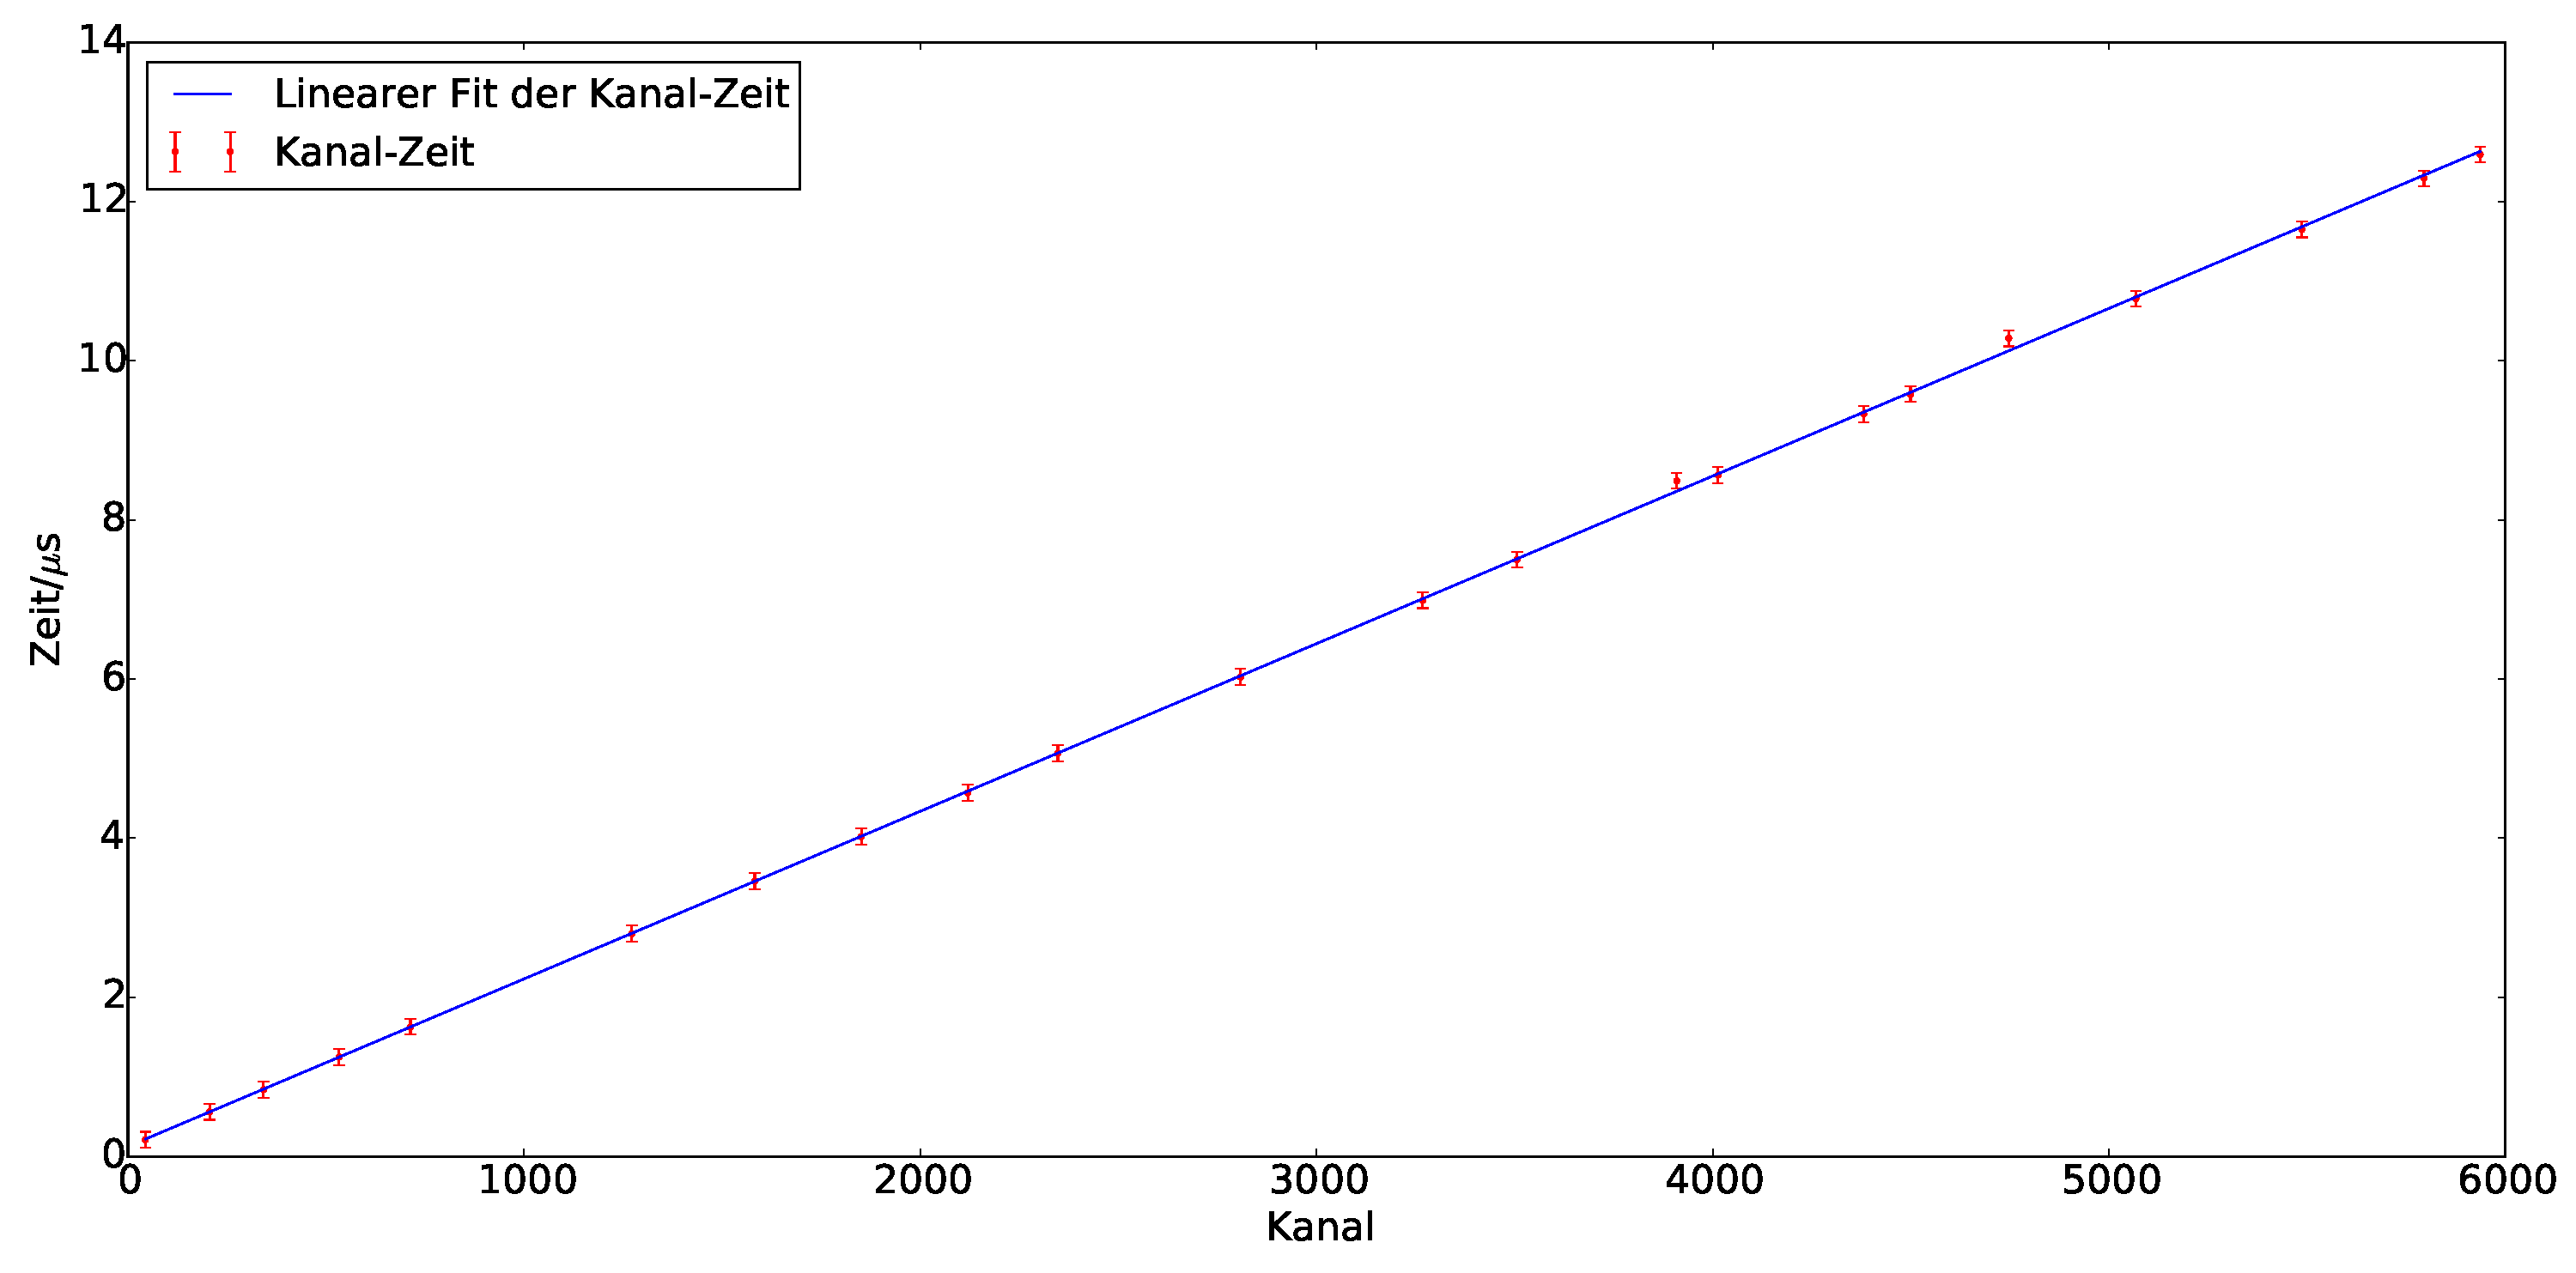
\includegraphics[scale=0.33]{kanal_zeitax+b.pdf} 
	\caption{Kanal-Zeit-Eichung}
	\label{fig:kanal_zeit_fit}
\end{figure}
Zum Vergleich sind die Fitparameter f�r $B = 0$ in Tabelle \ref{tab:fit2} zu sehen. Der Fit f�r $B = 0$ ist in Abb. \ref{fig:kanal_zeit_fit2} dargestellt.
\begin{table}[H]
\centering
\caption{Fitparameter mit Fehlern und $\chi_{red}^2$ f�r $B = 0$}
\label{tab:fit2}
\begin{tabular}{|c|c|}
\hline Paramter & Wert \\ 
\hline A & 0.002136(5) \\ 
\hline B & 0 \\ 
\hline $\chi_{red}^2$ & 0,719 \\ 
\hline 
\end{tabular} 
\end{table}
\begin{figure}[H] 
	\centering
	  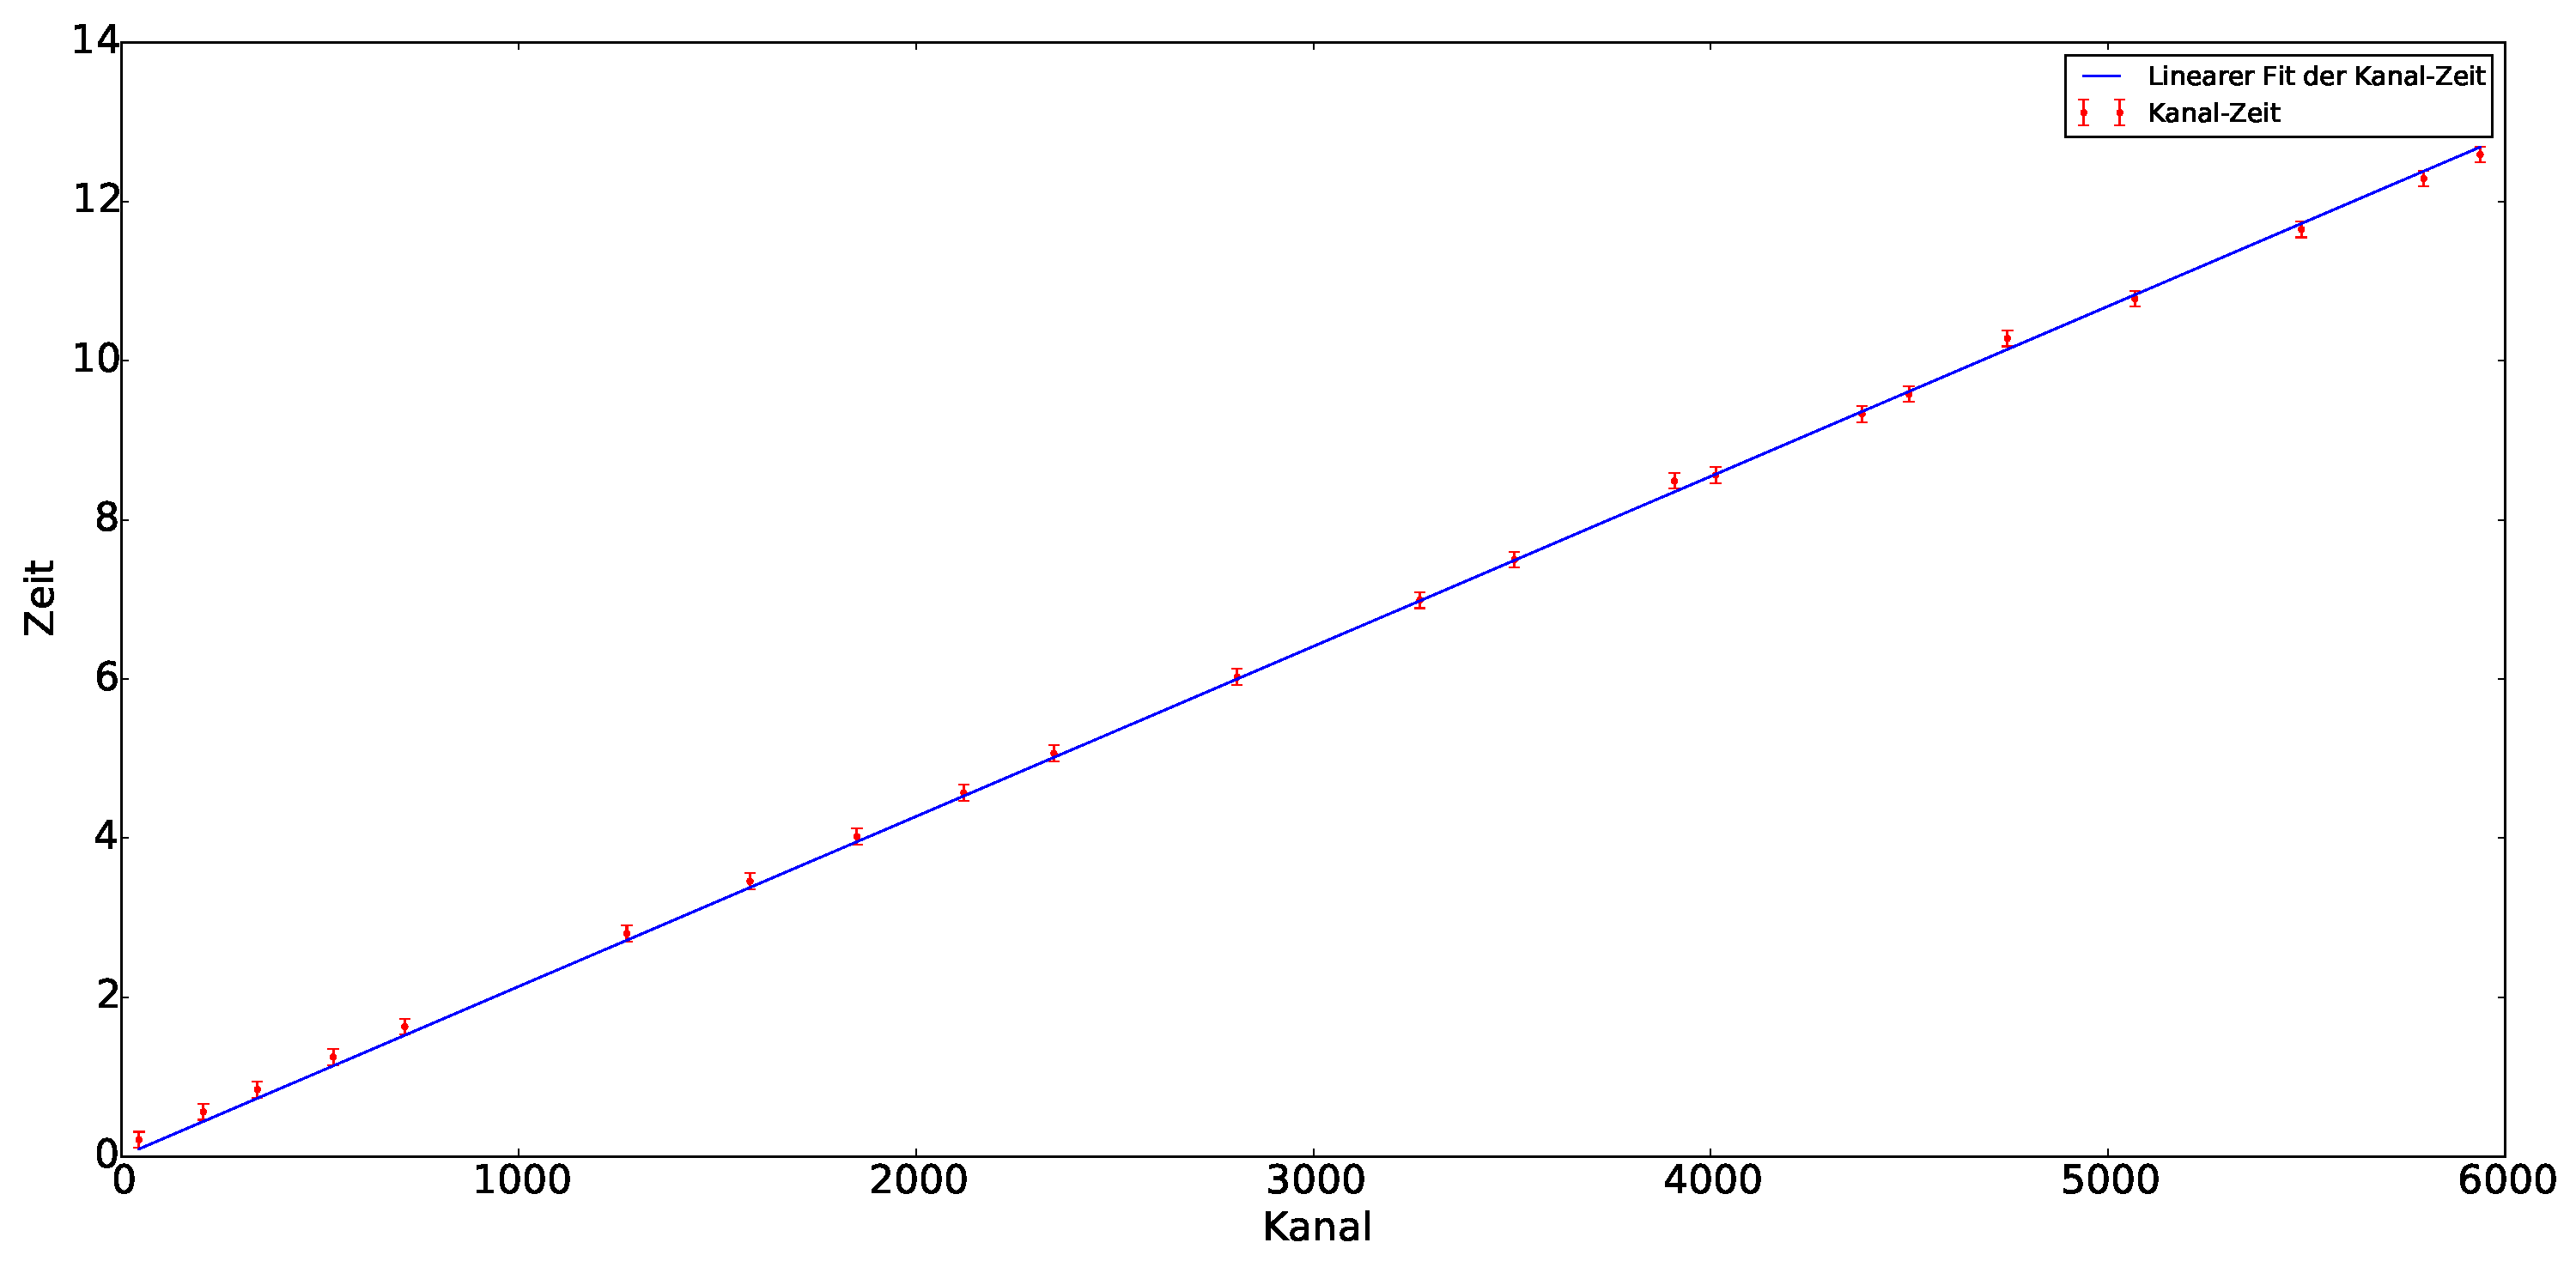
\includegraphics[scale=0.33]{kanal_zeitax.pdf} 
	\caption{Kanal-Zeit-Eichung f�r $B = 0$}
	\label{fig:kanal_zeit_fit2}
\end{figure}
\subsection{Messung der mittleren Lebensdauer}
Nachdem die umfangreichen Kalibrationen beendet sind, soll die Lebensdauer der Myonen anhand der Messdaten bestimmt werden. Dazu werden die folgenden Methoden verwendet und deren Resultat verglichen.
\subsubsection{Maximum Likelihood Methode}
Um die mittlere Lebensdauer von Myonen zu bestimmen eignet sich die Maximum Likelihood Methode. Wie in Abschnitt 2.3 besprochen sind Zerfallszeiten mit Zeitunabh�ngiger Zerfallsrate exponentialverteilt, sodass sich die einparametrige Warscheinlichkeitsdichte
\begin{align}
P(t_i|\tau) = \frac{1}{\tau}\frac{e^{-\frac{t_i}{\tau}}}{e^{-\frac{T_1}{\tau}}-e^{-\frac{T_2}{\tau}}}
\end{align}
ergibt. Da die Messung des Zeitintervalls nach oben und unten beschr�nkt ist, wurde die Warschenlichkeitsdichte normiert, wobei $T_1$ die untere Schranke und $T_2$ die obere Schranke der Zeitmessung ist. Es wird davon ausgegangen, dass die einzelnen Zeitmessungen unabh�ngig voneinander sind, sodass sich f�r die gesamte Messung die n-dimensionale Warscheinlichkeitsdichte
\begin{align}
L = \prod_{i=1}^N P(t_i|\tau) = \prod_{i=1}^N \frac{1}{\tau}\frac{e^{-\frac{t_i}{\tau}}}{e^{-\frac{T_1}{\tau}}-e^{-\frac{T_2}{\tau}}}
\end{align}
ergibt. Es wird davon ausgegangen, dass die gemessenen Zerfallszeiten der wahrscheinlichsten Messung entsprechen, sodass die Messung einem Maximum der Warscheinlichkeitsdichtefunktion bez�glich $\tau$ entspricht. Um das Maximum von $L$ zu bestimmen betrachtet man die Funktion
\begin{align}
\ln{L} = \ln\left[\prod_{i=1}^N P(t_i|\tau)\right] = \sum_{i=1}^{N}\ln[P(t_i|\tau)] = -\left[\sum_{i=1}^{N}\ln(\tau) + \frac{t_i}{\tau} + \ln(e^{-\frac{T_1}{\tau}}-e^{-\frac{T_2}{\tau}})\right]
\end{align}
und bestimmt die Nullstelle der Ableitung nach $\tau$.
Schlie�lich erh�lt man die beste Approximation f�r die Lebensdauer $\tau$:
\begin{align}
\hat{\tau} = \frac{1}{N}\sum_{i=1}^{N} t_i - \frac{T_1e^{-\frac{T_1}{\tau}}-T_2e^{-\frac{T_2}{\tau}}}{e^{-\frac{T_1}{\tau}}-e^{-\frac{T_2}{\tau}}}
\end{align}
Da es nur M Kan�le und damit M m�gliche Zeiten $t_k$ gibt, kann die erste Summe umgeschrieben werden,
\begin{align}
\sum_{i=1}^{N} t_i = \sum_{k=1}^{M} N_k t_k \text{ wobei } N = \sum_{k=1}^{M} N_k
\end{align}
sodass der Fehler von $\hat{\tau}$ �ber den statistischen Fehler auf $N_k$, welcher $\sqrt{N_k}$ betr�gt, bestimmt werden kann.
Es ergibt sich also
\begin{align}
\hat{\tau} = \sum_{k=1}^{M} N_k t_k - \frac{T_1e^{-\frac{T_1}{\tau}}-T_2e^{-\frac{T_2}{\tau}}}{e^{-\frac{T_1}{\tau}}-e^{-\frac{T_2}{\tau}}}
\end{align}
mit einem Fehler von
\begin{align}
\Delta\hat{\tau} = \frac{1}{N}\sqrt{\sum_{k=1}^{M}N_kt_k^2}
\end{align}

\section{Versuchsdurchf�hrung und Auswertung}
%die messwerte in !�bersichtlichen! tabellen angegeben
%zu viele kleine tabellen in gro�e tabellen �berf�hren!
%zu gro�e tabellen mit dem [scale]-befehl scalieren oder (falls zu lang) in zwei kleinere tabellen aufteilen
%(wichtig) vor !jeder! tabeelle sagen, was gemessen wurde und wie die fehler gew�hlt wurden und ausreichend !erkl�ren!, !warum! wir unsere fehler grade so gew�hlt haben

%zuerst !alle! errechneten werte entweder in ganzen s�tzen aufz�hlen, oder in tabellen (�bersichtlicher) dargestellen, sowie auf die verwendeten formeln verweisen (die referenzierung der formel kann in der �berschrift stehen)
%kurz erw�hnen (vor der tabelle), warum wir das ganze ausrechnen bzw. was wir dort ausrechnen
%danach histogramme und plots erstellen, wobei wenn m�glich funktionen durch die plots gelegt werden (zur not k�nnen auch splines benutzt werden, was aber angegeben werden muss)
%bei fits immer die funktion und das reduzierte chiquadrat mit angegeben, wobei auf verst�ndlichkeit beim entziffern der zehnerpotenzen geachtet werden muss z.b. f(x)=(wert+-fehler)\cdot10^{irgendeine zahl}\cdot x + (wert+-fehler)\cdot10^{irgendeine zahl}
%bei jedem fit erkl�ren, nach welchem zusammenhang gefittet wurde und warum!
%bei plots darauf achten, dass die achsenbeschriftung (auch die tics) die richtige gr��e haben und die legende im plot nicht die messwerte verdeckt
%kurz die aufgabenstellung abgehandeln

Der Versuch besteht aus f�nf Teile, welche im folgendem beschrieben und ausgewertet werden.

\subsection{Inbetriebnahme}
Vor dem einstellen des SQUID muss das Dewar-Gef�� in ein Bad von fl�ssigem Stickstoff getaucht werden, damit der Sensor nicht durch Feuchtigkeit zerst�rt wird und die Supraleitung nicht unterbrochen wird. Das Bad von fl�ssigem Stickstoff muss eventuell w�hrend dem Versuch nachgef�llt werden. Der Abk�hlprozess dauert ca. 20 min, danach k�nnen Messungen gestartet werden. Zu erst soll die Amplitude I$_{rf}$ (VCA, voltage controlled atteuator) und die Auslesefrequenz (VCO voltage controlled oscillator) des rf-Signals so ein maximales Signal-zu-Rausch-Verh�ltnis von U($\Phi$) erreicht wird. F�r die Einstellungen wird der Testmodus, mit eingeschaltetem Generator verwendet. Zu erst wird f�r VCA ein Werte von 900 eingestellt.
% Kapazit�ts- und Widerstandsangaben hinzuf�gen
Dann wird der VCO Wert zwischen 0 und 4095 so variiert, das m�glichst deutlich ein Dreiecksignal zu sehen ist. Der VCA Wert wird nun nochmal variiert um das Signal weiter zu optimieren.

%  Bild und die Werte einf�gen

F�r die Einstellung des Arbeitspunkts wird das Offsets kalibriert. Das SQUID wird im Messmodus betrieben um die zeitliche Magnetfeld�nderung auf dem Oszilloskop zu beobachten. Es wird ein Kompensations-Widerstand von 20k$\Omega$ gew�hlt. Falls das Offset richtig eingestellt ist sollten keine Peaks auf dem Oszilloskop zu sehen sein. Falls Peaks nach oben zu sehen sind, ist das Offset zu hoch eingestellt. Bei Peaks, die nach unten zeige, ist das Offset zu niedrig eingestellt.

% Auswertung + Bilder + weiterf�hrende Analysen(50Hz Rauschen)

\subsection{Empfindlichkeit des SQUID}
Zur Untersuchung der Empfindlichkeit wird das SQUID im Messmodus betrieben. Um einen ersten Eindruck der Empfindlichkeit zu bekommen wurde .......................................

% kurze beschreibund der beobachungen + Bilder

F�r eine quantitative Bestimmung der Empfindlichkeit des SQUIDs wurde mit einer Spule Magnetfelder bekannter st�rke erzeugt. Um bei der Messung eine m�glichst hohe Empfindlichkeit zu haben wird ein Widerstand von 20k$\Omega$ verwendet. 

% messergebnisse und auswertung

\subsection{Kalibrierung}
F�r die weiteren Messungen muss der Sensor zuerst kalibriert werden, um as dem Signal die st�rke des Magnetfeldes bestimmen zu k�nnen. Es soll auch die Empfindlichkeit des SQUID in Abh�ngigkeit des R�ckkopplungswiderstandes gemessen werden. Zuerst wird f�r einen festen Widerstand das Magnetfeld in Abh�ngigkeit der Str�me in der Leiterschleife untersucht. Es werden Str�me zwischen \SI{0}{mA} und \SI{90}{mA} verwendet. 

% messdaten und widerstand angeben

Aus den H�hen der Plateaus und den jeweiligen Str�men kann eine lineare Regerssion durchgef�hrt werden, um den Zusammenhang zwischen dem Strom in der Leiterschleife und der Spannung her zu stellen.

%messdaten + bilder

Die Messung wird f�r die anderen Widerst�nde wiederholt (siehe Abb. ??)

\subsection{Aufzug}
In diesem Versuchsteil soll das Magnetfeld der Aufz�ge untersucht werden. Dabei wird der Aufzug als Dipol angenommen, da das Gegengewicht eine nat�rliche Magnetisierung besitzt. Durch die Messung soll die z-Komponente des Dipols bestimmt werden.

\subsection{Magnetisierungskurve von Gadolinium und Curie-Temperatur}
In diesem Versuchsteil soll aus der Magnetisierungskurve von Gadolinium die Curie-Temperatur abgelesen werden. Zuerst wird das Gadolinium unter T$_c$ gek�hlt und magnetisiert. Die Temperatur wird dabei mit einem PT1000 Element gemessen.
\subsection{Diskussion}
%(immer) die gemessenen werte und die bestimmten werte �ber die messfehler mit literaturwerten oder untereinander vergleichen
%in welchem fehlerintervall des messwertes liegt der literaturwert oder der vergleichswert?
%wie ist der relative anteil des fehlers am messwert und damit die qualit�t unserer messung?
%in einem satz erkl�ren, wie gut unser fehler und damit unsere messung ist
%kurz erl�utern, wie systematische fehler unsere messung beeinflusst haben k�nnten
%(wichtig) zum schluss ansprechen, in wie weit die ergebnisse mit der theoretischen vorhersage �bereinstimmen
%--------------------------------------------------------------------------------------------
%falls tabellen mit den messwerten zu lang werden, kann die section mit den messwerten auch hinter der diskussion angef�gt bzw. eine section mit dem anhang eingef�gt werden.

Um die Diskussion konsistent zu halten, werden nur die Messdaten unserer Kommilitonen Diskutiert. 

Beim Sputtern wurden Prismen mit 5 verschiedenen Dicken Goldschichten erstellt 18nm, 27nm, 36nm, 45nm und 63nm. Bevor die Messung begonnen werde konnten, musste die Messapparatur justiert werden. Zuerst wurde die Position des Detektors justiert, dabei wurde eine Offset von 1,9(2) $^\circ$ bestimmt. Damit ergibt sich die Nulllage bei 181,9 $^\circ$. Bei der Bestimmung des Winkels, bei dem parallel bzw. senkrecht Polarisiertes Licht erzeugt wird, ergab sich ein Winkel von 89$^\circ$. Entsprechend ist der Winkel f�r senkrecht polarisiertes Licht -1$^\circ$. Der Brechungsindex des Prismas wurde �ber den Brewsterwinkel bestimmt, dabei ergab sich ein Wert von n$_{prisma}$=1.51. Nach der Justierung konnte die R$_p$/R$_s$-Kurve aufgenommen werden. Bei den allen Schichtdicken au�er der 63nm Schicht ist die Plasmonenresonanzkurve deutlich zu sehen. �ber eine Fit konnte der Resonanzwinkel bestimmt werden, aus welchem die Wellenzahl der Oberfl�chenplasmonen bestimmt werden konnte. Es ergab sich eine maximale Wellenzahl von 9,96(11) $\cdot$ 10$^6$ m$^{-1}$.


\section{Conclusion}
%im fazit nochmal alles zusammenfassen und den verlauf der messung absch�tzen
%gravierende sytematische probleme bei den messungen nochmal betonen und die wertigkeit unserer ergebnisse einordnen

In the first part of the experiment the 39 peaks of the nH$_3$ spectrum where measured and there relative absorption coefficients where calculated. In the second part the quadrupole moment where determined with a value of 5.02(9), with a deviation of 17.53\%. In the last part the broadening of the peaks according to the pressure was determined with 28 witch is a good measurement. 



%\bibliography{ref}

\end{document}